% !TeX root = ./beamer.tex
%%%%%%%%%%%%%%%%%%%%%%%%%%%%%%%%%%%%%%%%%%%%%%%%%%%%%%%%%%%%%%%%%%%%%%
% LaTeX Template: Beamer arrows
%
% Source: http://www.texample.net/
% Feel free to distribute this template, but please keep the
% referal to TeXample.net.
% Date: Nov 2006
%
%%%%%%%%%%%%%%%%%%%%%%%%%%%%%%%%%%%%%%%%%%%%%%%%%%%%%%%%%%%%%%%%%%%%%%
% How to use writeLaTeX:
%
% You edit the source code here on the left, and the preview on the
% right shows you the result within a few seconds.
%
% Bookmark this page and share the URL with your co-authors. They can
% edit at the same time!
%
% You can upload figures, bibliographies, custom classes and
% styles using the files menu.
%
% If you're new to LaTeX, the wikibook is a great place to start:
% http://en.wikibooks.org/wiki/LaTeX
%
%%%%%%%%%%%%%%%%%%%%%%%%%%%%%%%%%%%%%%%%%%%%%%%%%%%%%%%%%%%%%%%%%%%%%%

\documentclass[xcolor=dvipsnames]{beamer} %
\usetheme[progressbar=frametitle,
    titleformat=smallcaps,
    % sectionpage=none,
    numbering=fraction,
    block=fill,
    background=dark]{metropolis}
% \usepackage[latin1]{inputenc}
\usefonttheme{professionalfonts}
\usefonttheme{serif} % default family is serif
\usepackage{times}
\usepackage{tikz}
\newcommand{\dt}[1][t]{\mathrm{d}#1}

\usepackage{amsmath,amsfonts,amssymb,amsthm,mathtools}
\usepackage{subcaption}
\usepackage{copyrightbox}
\makeatletter
\renewcommand{\CRB@setcopyrightfont}{%
\color{black!33}
\usefonttheme{serif}\selectfont
}
\makeatother
% \captionsetup{justification=centering, labelfont=sc, labelsep=endash}
\usepackage{movie15}
\usepackage{animate}
\usepackage{multimedia}
\usepackage{wrapfig}
\usepackage[backend=biber,style=numeric]{biblatex}
% \usepackage[backend=biber,style=ieee]{biblatex}
\addbibresource{/home/een023/science/ref/ref.bib}
\addbibresource{ref.bib}
\usepackage{natbib}
\usepackage{multicol}
\usepackage{pgf,pgfpages}
\usepackage{graphicx}
\usepackage[version=4]{mhchem}
\usepackage[utf8]{inputenc}\DeclareUnicodeCharacter{2212}{-}
\newcommand{\inputpgf}[2][1]{
  \resizebox{#1\linewidth}{!}{%
  \input{#2}
  }%
}
\usepackage{appendixnumberbeamer}
\DeclareMathOperator{\sech}{sech}
\setbeamertemplate{note page}{\pagecolor{yellow!5}\vfill\insertnote\vfill}
% \setbeameroption{show only notes} % Only notes
% \setbeameroption{show notes on second screen=right} % Both

% %%%%%%%%%%%%%%%%%% New UiT colors %%%%%%%%%%%%%%%%%%
% UiT color palette: https://uit.no/ressurs/uit/profil2019/examples/fargekart.png
\definecolor{MainBlue}{HTML}{003349} % #003349
\definecolor{LightBlue}{HTML}{007396} % #007396
\definecolor{DarkBlue}{HTML}{102064} % #102174
\definecolor{Orange}{HTML}{f2a900} % #f2a900
\definecolor{Red}{HTML}{cb333b} % #cb333b
% \usepackage{xcolor}
% \definecolor{astral}{RGB}{46,116,181} % rgb(46%,116%,181%)
\definecolor{dark-gray}{gray}{0.5}
\definecolor{light-gray}{gray}{0.8}
\setbeamercolor{progress bar}{fg=Orange, bg=LightBlue}
\setbeamercolor{title}{fg=light-gray}
\setbeamercolor{background canvas}{bg=MainBlue}
\setbeamercolor{section title}{fg=white,bg=red!50!black}
\setbeamercolor{alerted text}{fg=Orange, bg=DarkBlue}
\setbeamercolor{footnote}{fg=black!33}
\usepackage{verbatim}
\usetikzlibrary{arrows,shapes}
\usepackage{booktabs}
% To make a text box
\usepackage[absolute,overlay]{textpos}
\newcommand{\gf}[1]{\boldsymbol{#1}}

%%%%%%%%%%%%%%%%%%%
% This divides the TOC in the headline into two columns
% https://tex.stackexchange.com/questions/47939/beamer-with-warsaw-theme-two-column-navigation
\makeatletter
\def\insertsectionnavigation#1{%
  \hbox to #1{\vbox{{\usebeamerfont{section in head/foot}%
     \usebeamercolor[fg]{section in head/foot}%
     \def\slideentry##1##2##3##4##5##6{}%
     \def\sectionentry##1##2##3##4##5{%
       \ifnum##5=\c@part%
       \def\insertsectionhead{##2\hskip3em}%
       \def\insertsectionheadnumber{##1}%
       \def\insertpartheadnumber{##5}%
         \hyperlink{Navigation##3}{%
             \ifnum\c@section=##1%
               {\usebeamertemplate{section in head/foot}}%
             \else%
               {\usebeamertemplate{section in head/foot shaded}}%
             \fi%
         }\par
       \fi}%
       \parbox[c][0cm][c]{.5\paperwidth}{%
       \begin{multicols}{2}
       \dohead
       \end{multicols}}\space}
     }%
  \hfil}%
}

\def\insertsubsectionnavigation#1{%
  \hbox to #1{%
    \vbox{{%
      \usebeamerfont{subsection in head/foot}\usebeamercolor[fg]{subsection in head/foot}%
      \vskip0.5625ex%
      \beamer@currentsubsection=0%
      \def\sectionentry##1##2##3##4##5{}%
      \def\slideentry##1##2##3##4##5##6{\ifnum##6=\c@part\ifnum##1=\c@section%
        \ifnum##2>\beamer@currentsubsection%
        \beamer@currentsubsection=##2%
        \def\insertsubsectionhead{##5}%
        \def\insertsectionheadnumber{##1}%
        \def\insertsubsectionheadnumber{##2}%
        \def\insertpartheadnumber{##6}%
        \beamer@link(##4){%
              \ifnum\c@subsection=##2%
                {\usebeamertemplate{subsection in head/foot}}%
              \else%
                {\usebeamertemplate{subsection in head/foot shaded}}%
              \fi\hfill}\par
        \fi\fi\fi}%
       \hspace*{3em}\parbox[c][0cm][c]{\dimexpr.5\paperwidth-1em\relax}{%
       \begin{multicols}{2}
       \dohead\vskip0.5625ex\end{multicols}
       }\space
   }\hfil
}}}

\setbeamertemplate{headline}
{%
  \leavevmode\@tempdimb=2.4375ex%
  \ifnum\beamer@subsectionmax<\beamer@sectionmax%
    \multiply\@tempdimb by\beamer@sectionmax%
  \else%
    \multiply\@tempdimb by\beamer@subsectionmax%
  \fi%
  \ifdim\@tempdimb>0pt%
    \advance\@tempdimb by 1.125ex%
    \begin{beamercolorbox}[wd=.5\paperwidth,ht=0.5\@tempdimb,dp=2ex]{section in head/foot}%
      \vbox to0.5\@tempdimb{\vfill\insertsectionnavigation{.5\paperwidth}\vfill}%
    \end{beamercolorbox}%
    \begin{beamercolorbox}[wd=.5\paperwidth,ht=0.5\@tempdimb,dp=2ex]{subsection in head/foot}%
      \vbox to0.5\@tempdimb{\vfill\insertsubsectionnavigation{.5\paperwidth}\vfill}%
    \end{beamercolorbox}%
  \fi%
}
\makeatother
%%%%%%%%%%%%%%%%%%%

\makeatletter
\setlength{\metropolis@frametitle@padding}{.8ex}% <- default 2.2 ex

\setbeamertemplate{footline}{%
  \begin{beamercolorbox}[wd=\textwidth, sep=1.ex]{footline}% <- default 3ex
    \usebeamerfont{page number in head/foot}%
    \usebeamertemplate*{frame footer}
    \hfill%
    \usebeamertemplate*{frame numbering}
  \end{beamercolorbox}%
}
\makeatother
\usepackage{beamerouterthemesplit}
\setbeamerfont{footnote}{size=\tiny}

%%%%%%%%%%%%%%%%%%%
\let\svthefootnote\thefootnote

\makeatletter
% https://tex.stackexchange.com/a/29931/38244
\DeclareCiteCommand{\figurecite}
{\usebibmacro{prenote}}%
{%
    \ifciteseen{}{%
        \usebibmacro{citeindex}%
        \let\thefootnote\relax%
        \footnotetext{%
            \blx@anchor
            \mkbibbrackets{\usebibmacro{cite}}%
            \setunit{\addnbspace}
            \printnames{labelname}%
            \setunit{\labelnamepunct}
            \printfield[citetitle]{title}%
            \newunit%
            \printfield[]{year}%
        }%
        \let\thefootnote\svthefootnote%
    }%
    % \autocite{\thefield{entrykey}}%
}
{\addsemicolon\space}
{\usebibmacro{postnote}}
\makeatother
\makeatletter
% https://tex.stackexchange.com/a/29931/38244
\DeclareCiteCommand{\cite}
{\usebibmacro{prenote}}%
{%
    \ifciteseen{}{%
        \usebibmacro{citeindex}%
        \let\thefootnote\relax%
        \footnotetext{%
            \blx@anchor
            \mkbibbrackets{\usebibmacro{cite}}%
            \setunit{\addnbspace}
            \printnames{labelname}%
            \setunit{\labelnamepunct}
            \printfield[citetitle]{title}%
            \newunit%
            \printfield[]{year}%
        }%
        \let\thefootnote\svthefootnote%
    }%
    \autocite{\thefield{entrykey}}%
}
{\addsemicolon\space}
{\usebibmacro{postnote}}
\makeatother

%%%% Add unnumbered footnote command
\newcommand\blfootnote[1]{%
\begingroup
\renewcommand\thefootnote{}\footnote{#1}%
\addtocounter{footnote}{-1}%
\endgroup
}
%%%%%%%%%%%%%%%%%%%

\title{Estimating Temperature Response to Volcanic Eruptions}
\author[\textsc{Eirik Rolland Enger}]{\textsc{Eirik Rolland Enger}} %\\ Audun Theodorsen\\ Martin Rypdal}}
\date{\vspace{-3mm}\today\hfill
\includegraphics[width=4cm]{UiT_Logo_Eng_2l_Hvit.png}}
% \institute{UiT --- The Arctic University of Norway}
\logo{\vspace{-2mm}
\includegraphics[width=15mm]{UiT_Logo_Eng_2l_Hvit.png}\hspace{1mm}}
% Prevent footnotes to bleed over the logo
\newcommand{\beamerfoottmplength}{.78\paperwidth}
\addtobeamertemplate{footnote}{\hsize\beamerfoottmplength}{}
% \logo{text \raisebox{-0.5cm}{
\includegraphics[width=1cm]{UiT_Logo_Eng_2l_Hvit.png}}\hspace*{\textwidth}}
\begin{document}
% \maketitle
\begin{frame}[plain]
  \titlepage

  \note{
  \begin{itemize}
    \item ``Estimating Temperature Response to Volcanic Eruptions'' is
      hopefully insteresting, but I want to motivate this anyways.
  \end{itemize}
  }

\end{frame}
\setcounter{framenumber}{0}

\begin{comment}
:Title: Beamer arrows
:Tags: Remember picture, Beamer, Physics & chemistry, Overlays
:Use page: 3

With PGF/TikZ version 1.09 and later, it is possible to draw paths between nodes across
different pictures. This is a useful feature for presentations with the
Beamer package. In this example I've combined the new PGF/TikZ's overlay feature
with Beamer overlays. Download the PDF version to see the result.

**Note.** This only works with PDFTeX, and you have to run PDFTeX twice.

| Author: Kjell Magne Fauske
\end{comment}

% For every picture that defines or uses external nodes, you'll have to
% apply the 'remember picture' style. To avoid some typing, we'll apply
% the style to all pictures.
 \tikzset{
    invisible/.style={opacity=0,text opacity=0},
    visible on/.style={alt={#1{}{invisible}}},
    alt/.code args={<#1>#2#3}{%
      \alt<#1>{\pgfkeysalso{#2}}{\pgfkeysalso{#3}} % \pgfkeysalso doesn't change the path
    },
  }
\tikzstyle{every picture}+=[remember picture]

% By default all math in TikZ nodes are set in inline mode. Change this to
% displaystyle so that we don't get small fractions.
\everymath{\displaystyle}
% \begin{frame}%,[allowframebreaks]
%   \frametitle{Overview}

%   \setbeamertemplate{section in toc}[sections numbered]
%   \tableofcontents[hideallsubsections]

% \end{frame}

\section{Introduction}
\subsection{Motivation}

\begin{frame}{Equilibrium climate sensitivity (ECS)}

    Simple energy balance model:
    \begin{equation}
        C\frac{\mathrm{d}\Delta T}{\mathrm{d}t}=-\frac{1}{s}\Delta T+f
    \end{equation}

    \vspace{-7mm}
    \visible<2>{
        \begin{equation*}
            \downarrow
        \end{equation*}
        \begin{equation}
            \Delta T=sf_{2\times\ce{CO2}}
        \end{equation}

    \(\Delta T\sim\) Equilibrium climate sensitivity (ECS)
    }

    \note<+>{
        \begin{itemize}
            \item Starting with very simple linear EBM
        \end{itemize}
    }
    \note<+>{
        \begin{itemize}
            \item (Equilibrium) Climate sensitivity is a measure of temperature
                change to a radiative imbalance
            \item Large \(\rightarrow\) strong response to forcing and large temperature change,
                small \(\rightarrow\) modest response and small temperature change
            \item Robust feature of sophisticated models for different forcings. To
                first order the magnitude of the forcing is what matter, not the
                type (e.g.\ infrared vs.\ shortwave)
            \item Gives a simple measure of the severity of global warming
        \end{itemize}
    }

\end{frame}

\begin{frame}{Estimating ECS}

    \begin{figure}
        \centering
        \begin{tikzpicture}
            \node[anchor=south west,inner sep=0] at (0,0) {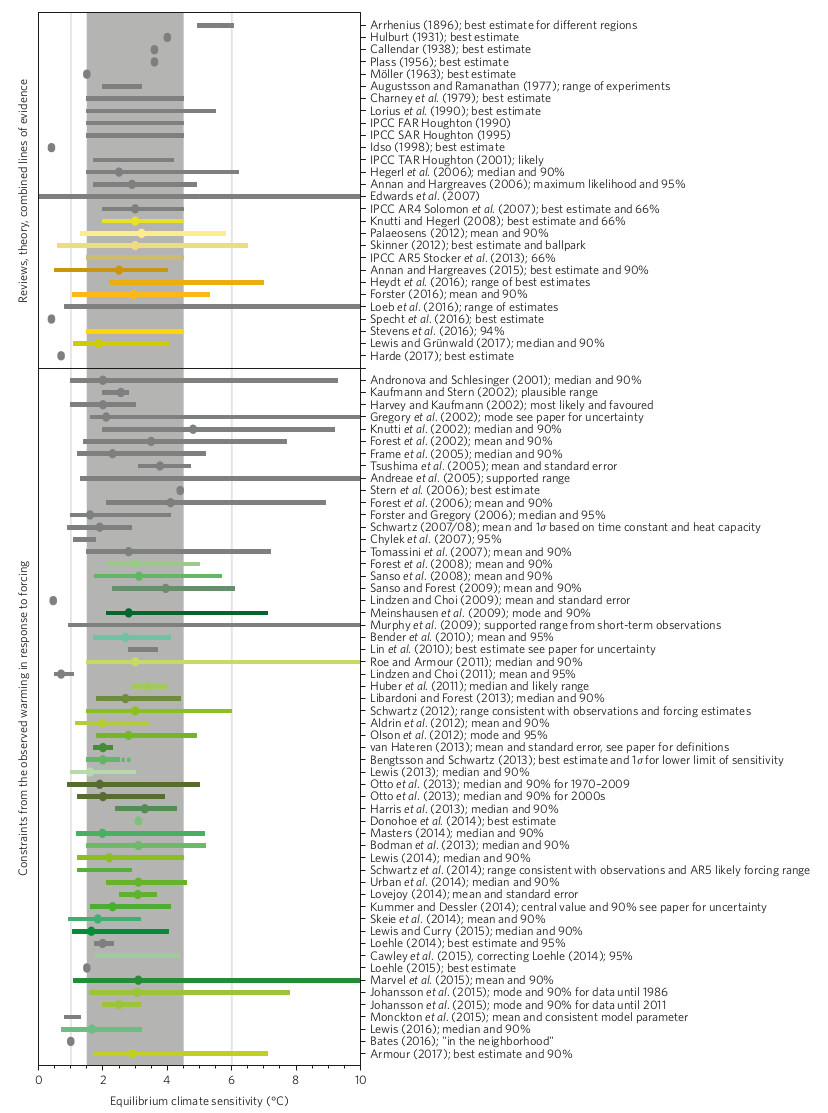
\includegraphics[width=.4\linewidth]{pic/equilibrium_climate_sensitivity.png}};
            \draw[white,anchor=south west,fill] (0.1,0.02) rectangle (1.6,0.1);
            \node[red,anchor=south west,inner sep=0] at (2.1,0.0) {\scalebox{.4}{ECS ($\mathrm{^\circ C}$)}};
            \node[red,anchor=south west,inner sep=0] at (0.16,0.02) {\scalebox{.4}{$0$}};
            \node[red,anchor=south west,inner sep=0] at (0.35,0.02) {\scalebox{.4}{$1.5$}};
            \node[red,anchor=south west,inner sep=0] at (0.85,0.02) {\scalebox{.4}{$4.5$}};
            \node[red,anchor=south west,inner sep=0] at (1.83,0.02) {\scalebox{.4}{$10$}};
        \end{tikzpicture}
        % 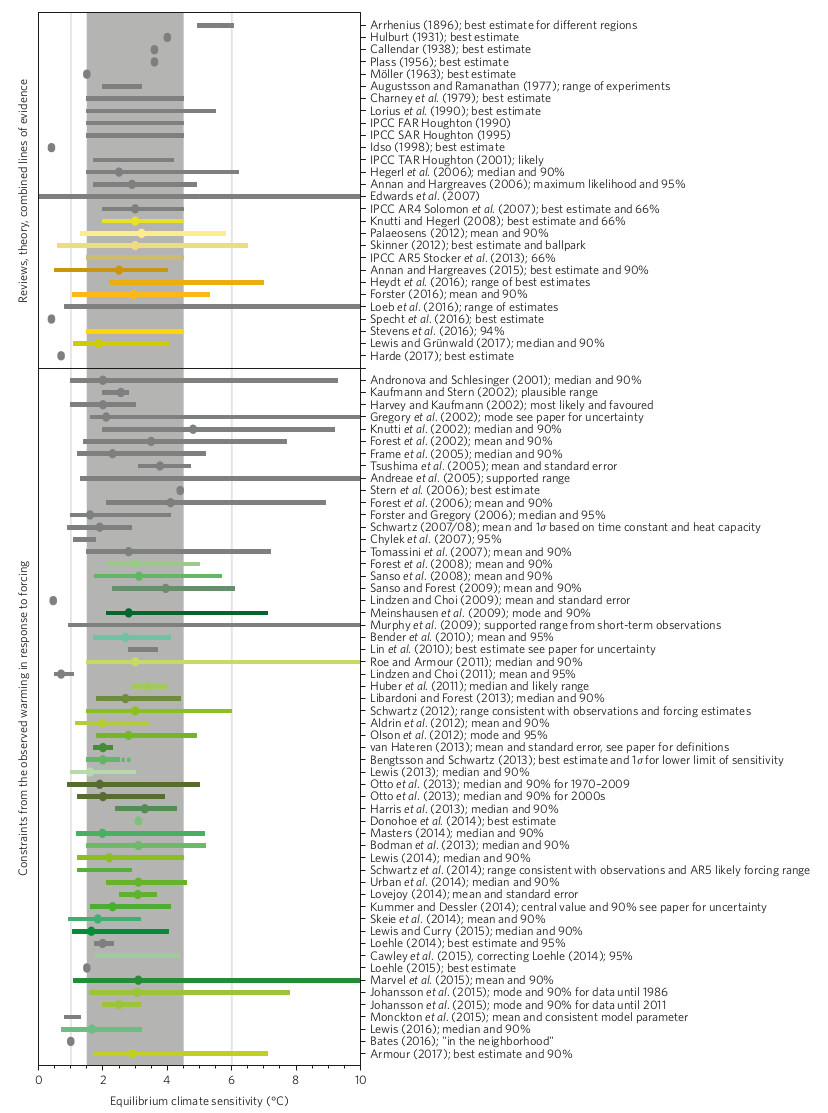
\includegraphics[width=.4\linewidth]{pic/equilibrium_climate_sensitivity.png}
        % 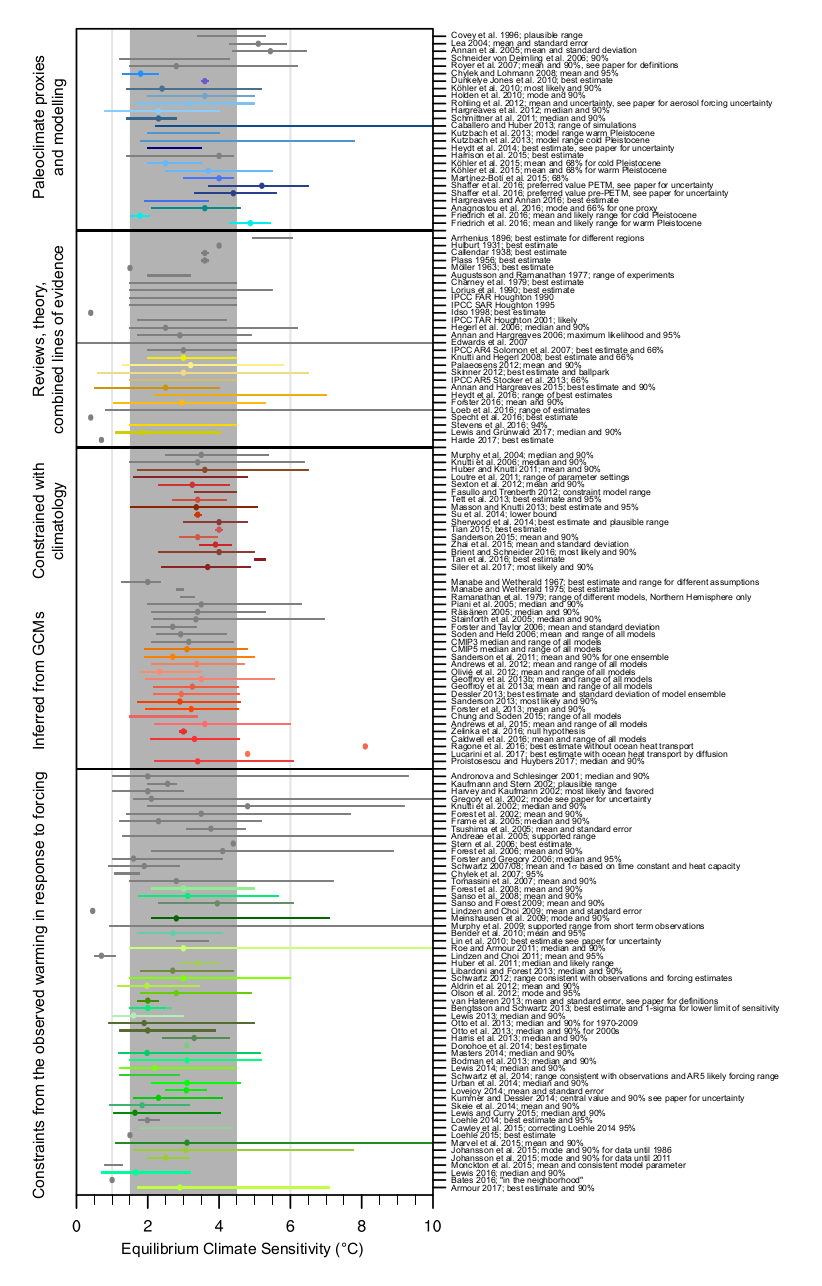
\includegraphics[width=.35\linewidth]{pic/ecs_supp_table.png}
        % \animategraphics[loop,autoplay,width=.5\linewidth]{2}{gif/volcanoe/volcanoe_}{0}{3}
        \visible<2>{
            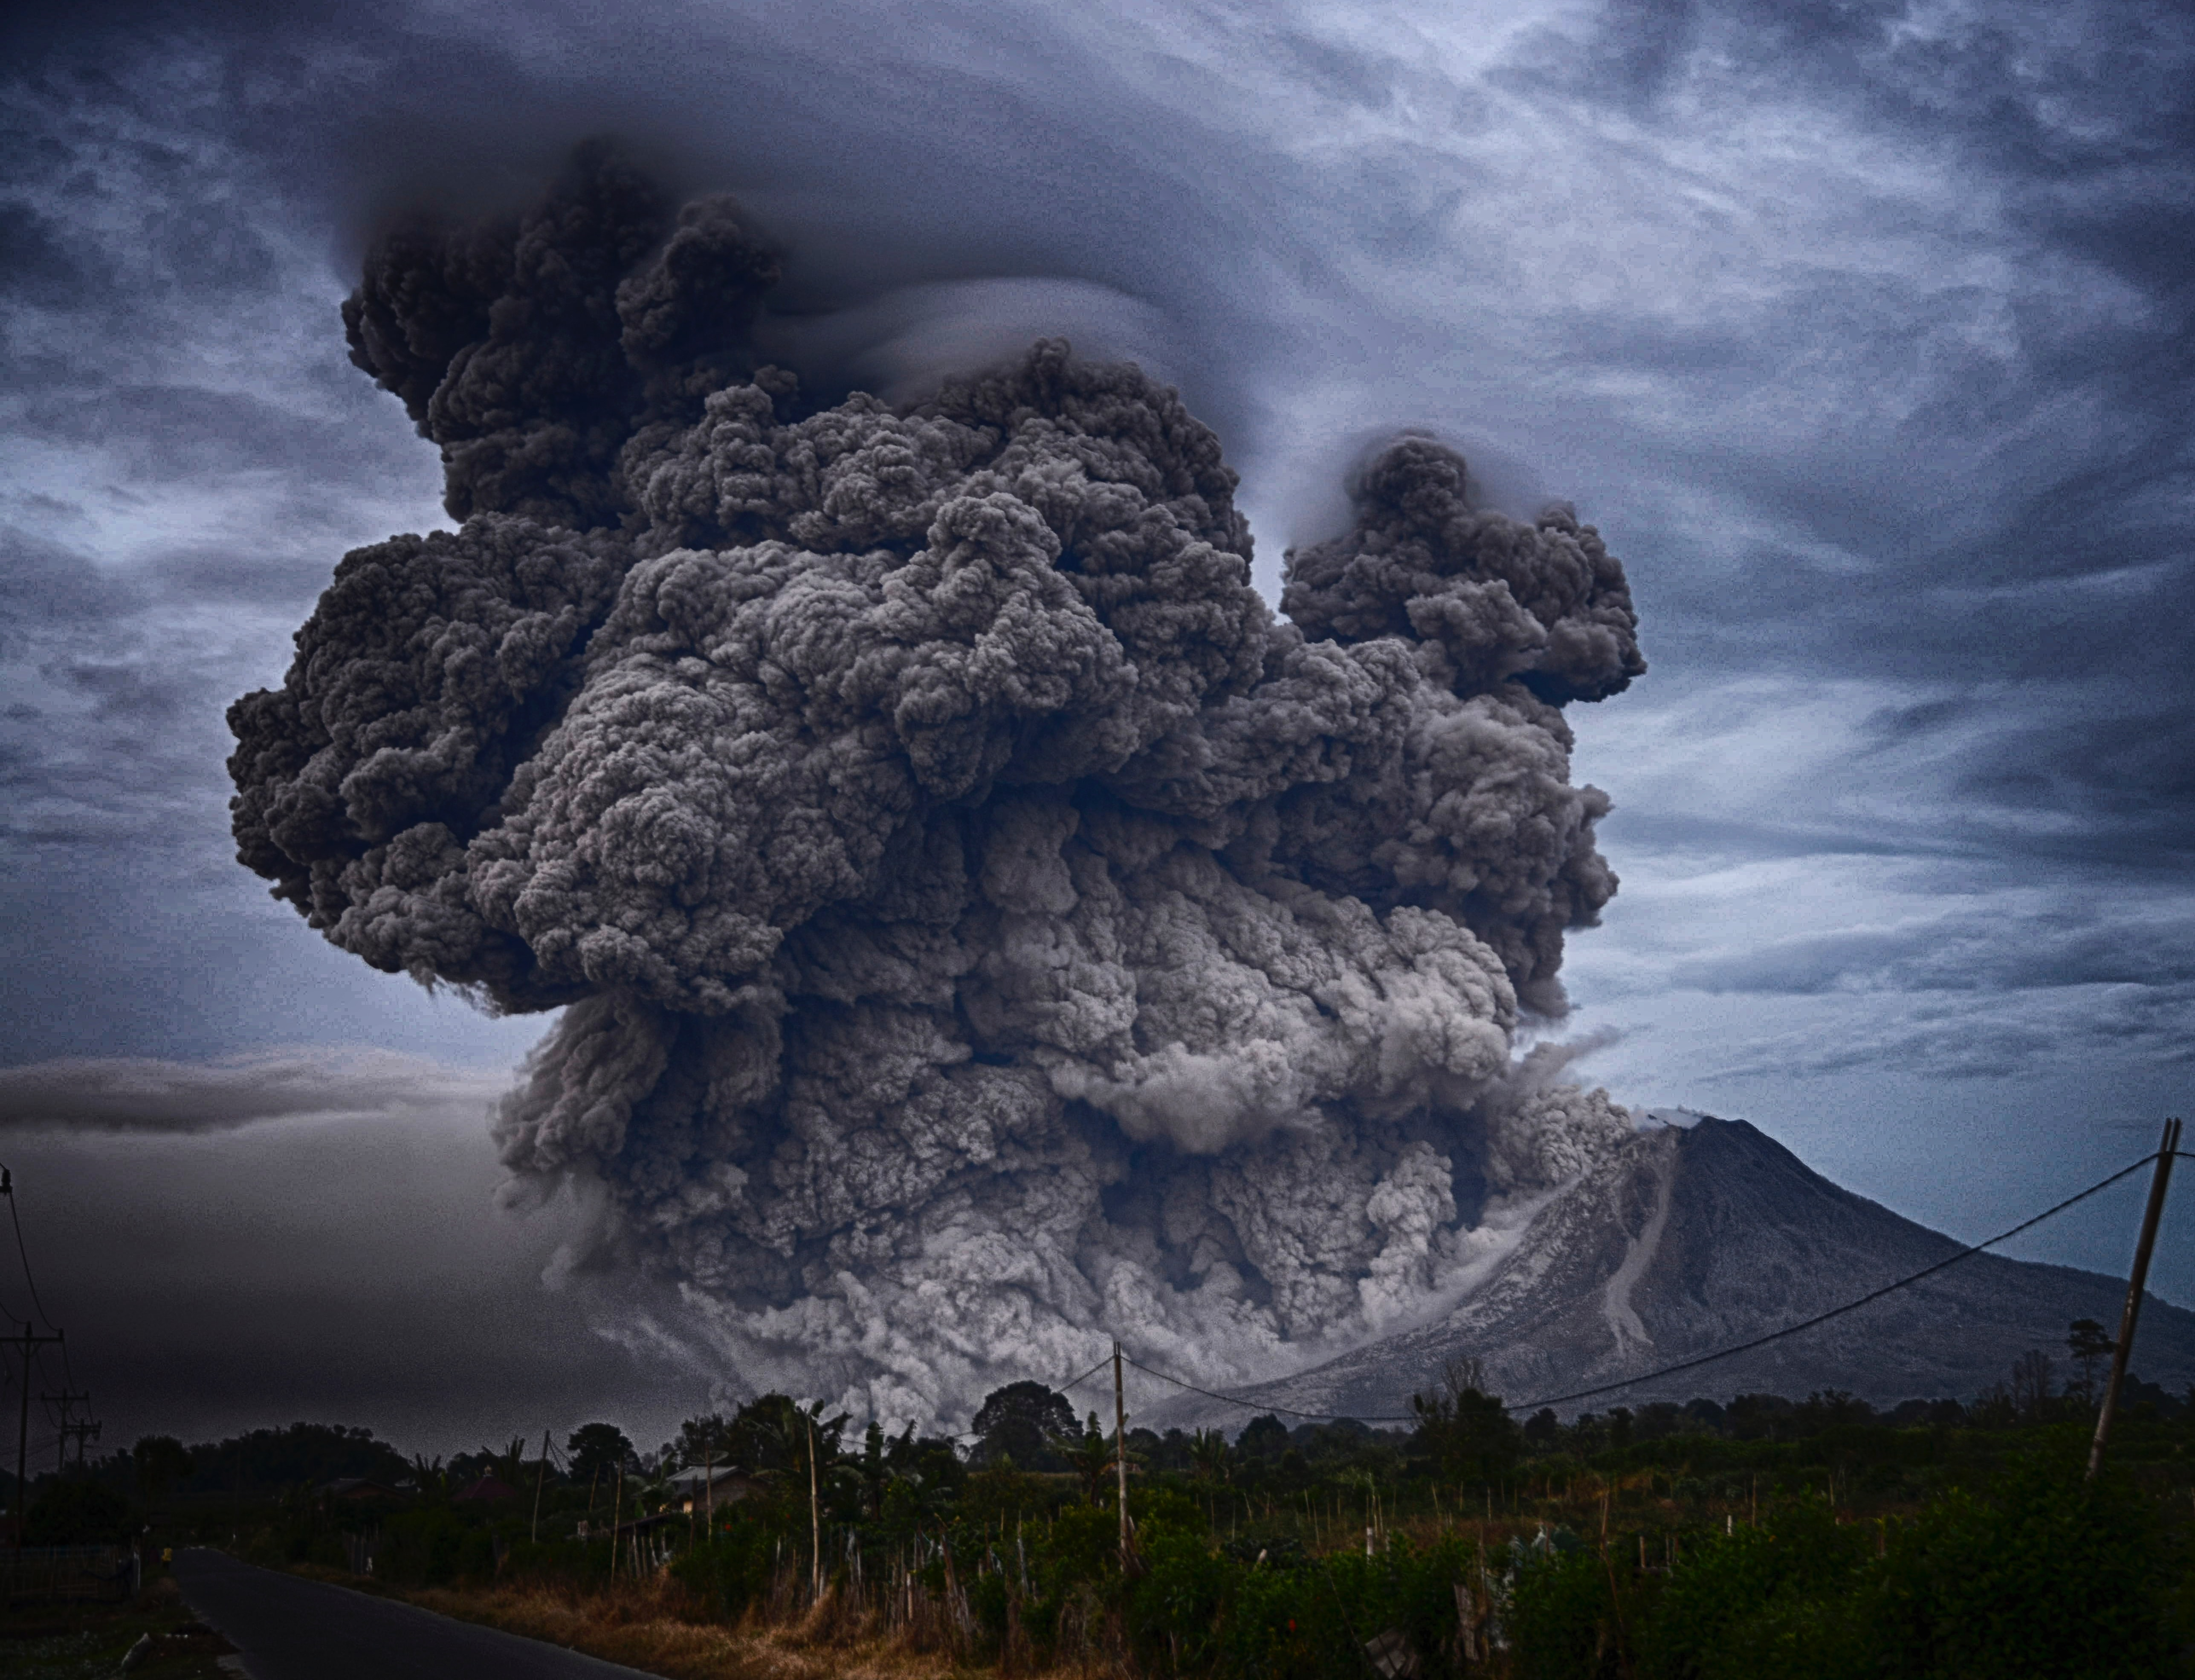
\includegraphics[width=.5\linewidth]{unsplash/volcano-unsplash.jpg}
            % 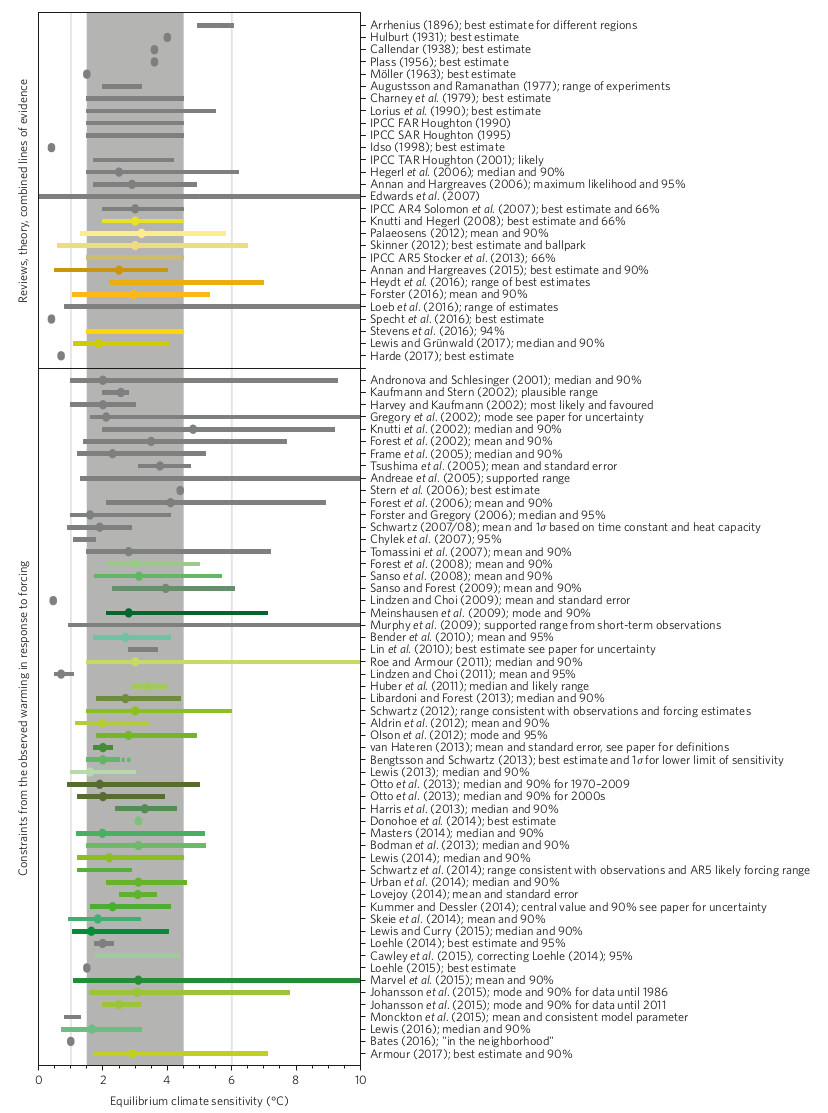
\includegraphics[width=.4\linewidth]{pic/equilibrium_climate_sensitivity.png}
        }
    \end{figure}
    \figurecite{knutti2017}

    \note<+>{
        \begin{itemize}
            \item On the right: each line is one paper/study
            \item On the left: best estimate of ECS from given study, with range in
                horisontal from 0 to 10
            \item IPCC ``likely'' region from 1.5 to 4.5
            \item Conclusion: it is difficult and literature do not agree,
                therefore, different methods are used, e.g. volcanoes
        \end{itemize}
    }
    \note<+>{
        \begin{itemize}
            \item ``Compared to anthropogenic and other natural forcings in the
                climate system, the volcanic radiative forcing acts on an short
                time scale, making the forcing and the proceeding system response
                comparatively easy to observe.''
        \end{itemize}
    }

\end{frame}

\subsection{Key points}

\begin{frame}{Key points}

    \begin{itemize}
        \item Estimate global temperature response and climate sensitivity
        \item Volcanoes produce strong temperature fluctuations
        \item Non-parametric approach
    \end{itemize}

    \note{
        \begin{itemize}
            \item Want to estimate global temperature response to volcanic
                eruptions, and possibly also climate sensitivity
            \item We know volcanoes produce strong temperature fluctuations and
                aim to infer the response from these eruptions
            \item How is this work different from other approaches? This is
                done using a non-parametric approach
        \end{itemize}
    }

\end{frame}


% \section{Model}
% \subsection{Filtered Poisson process}

\begin{frame}{Filtered Poisson process --- Examples}

    The FPP model intermittent processes:\vspace{-13mm}
    \begin{figure}
        \centering
        \visible<2->{
            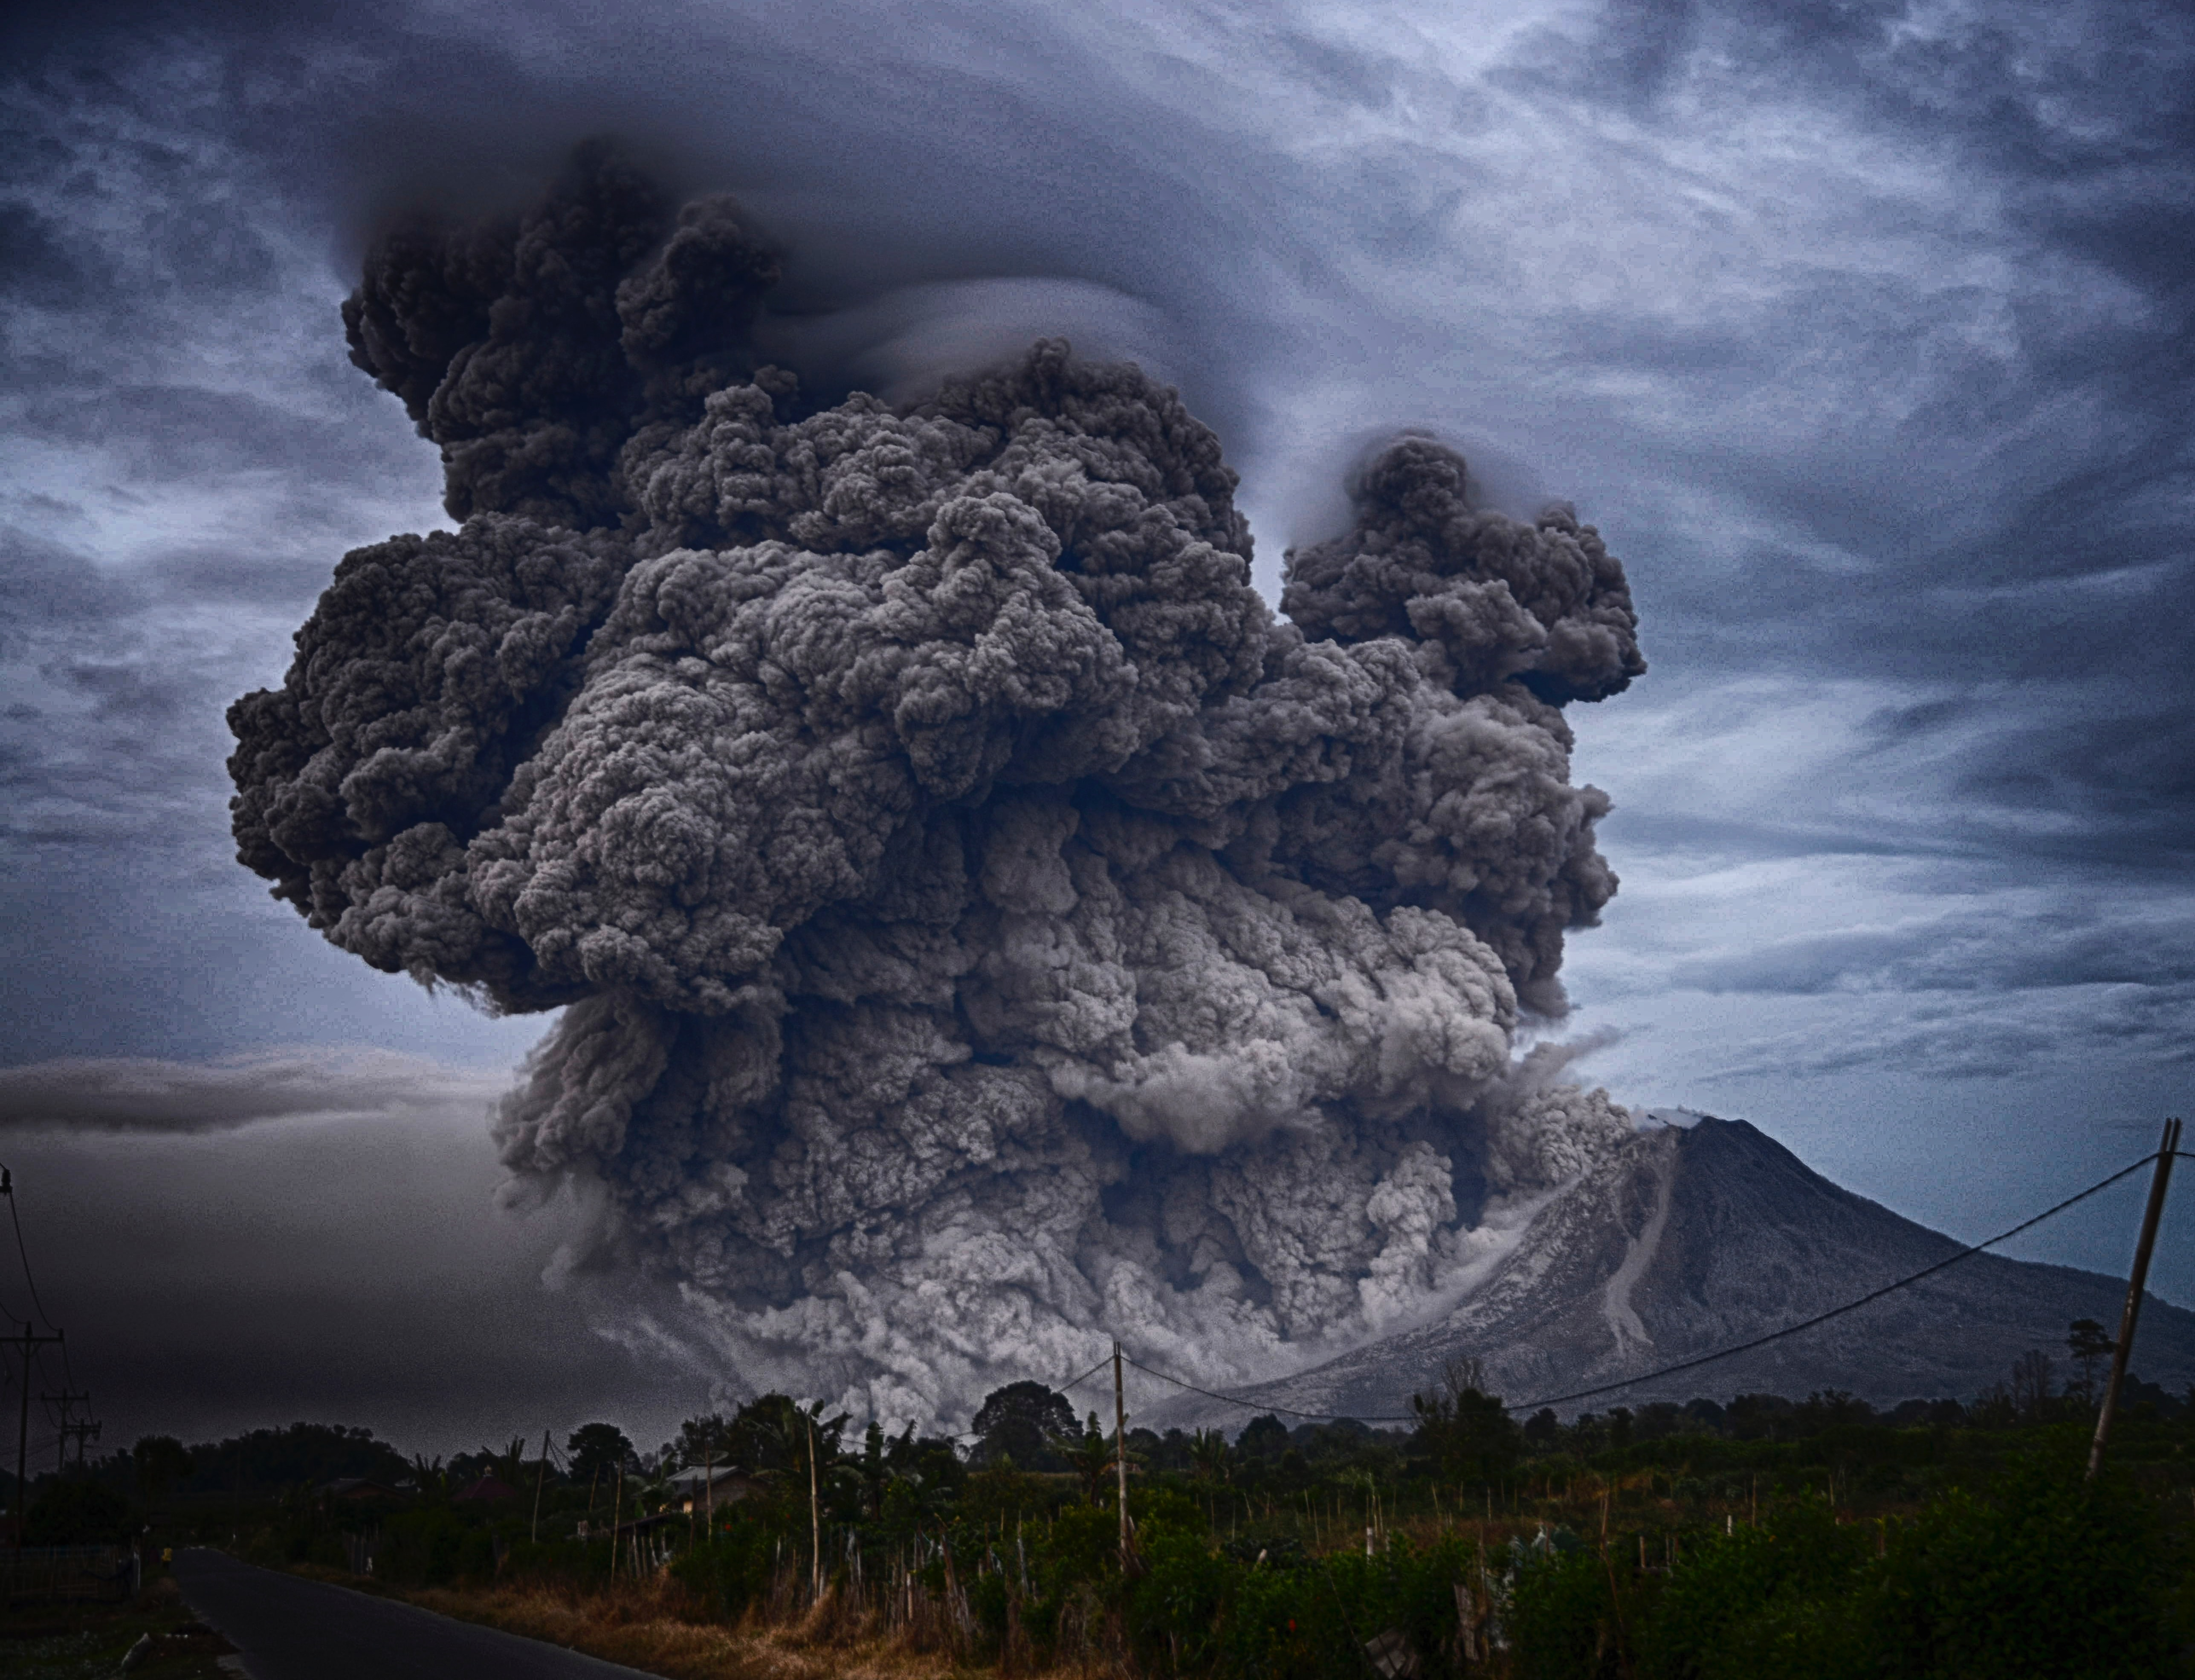
\includegraphics[width=.31\linewidth]{unsplash/volcano-unsplash.jpg}
        }
        \visible<3->{
            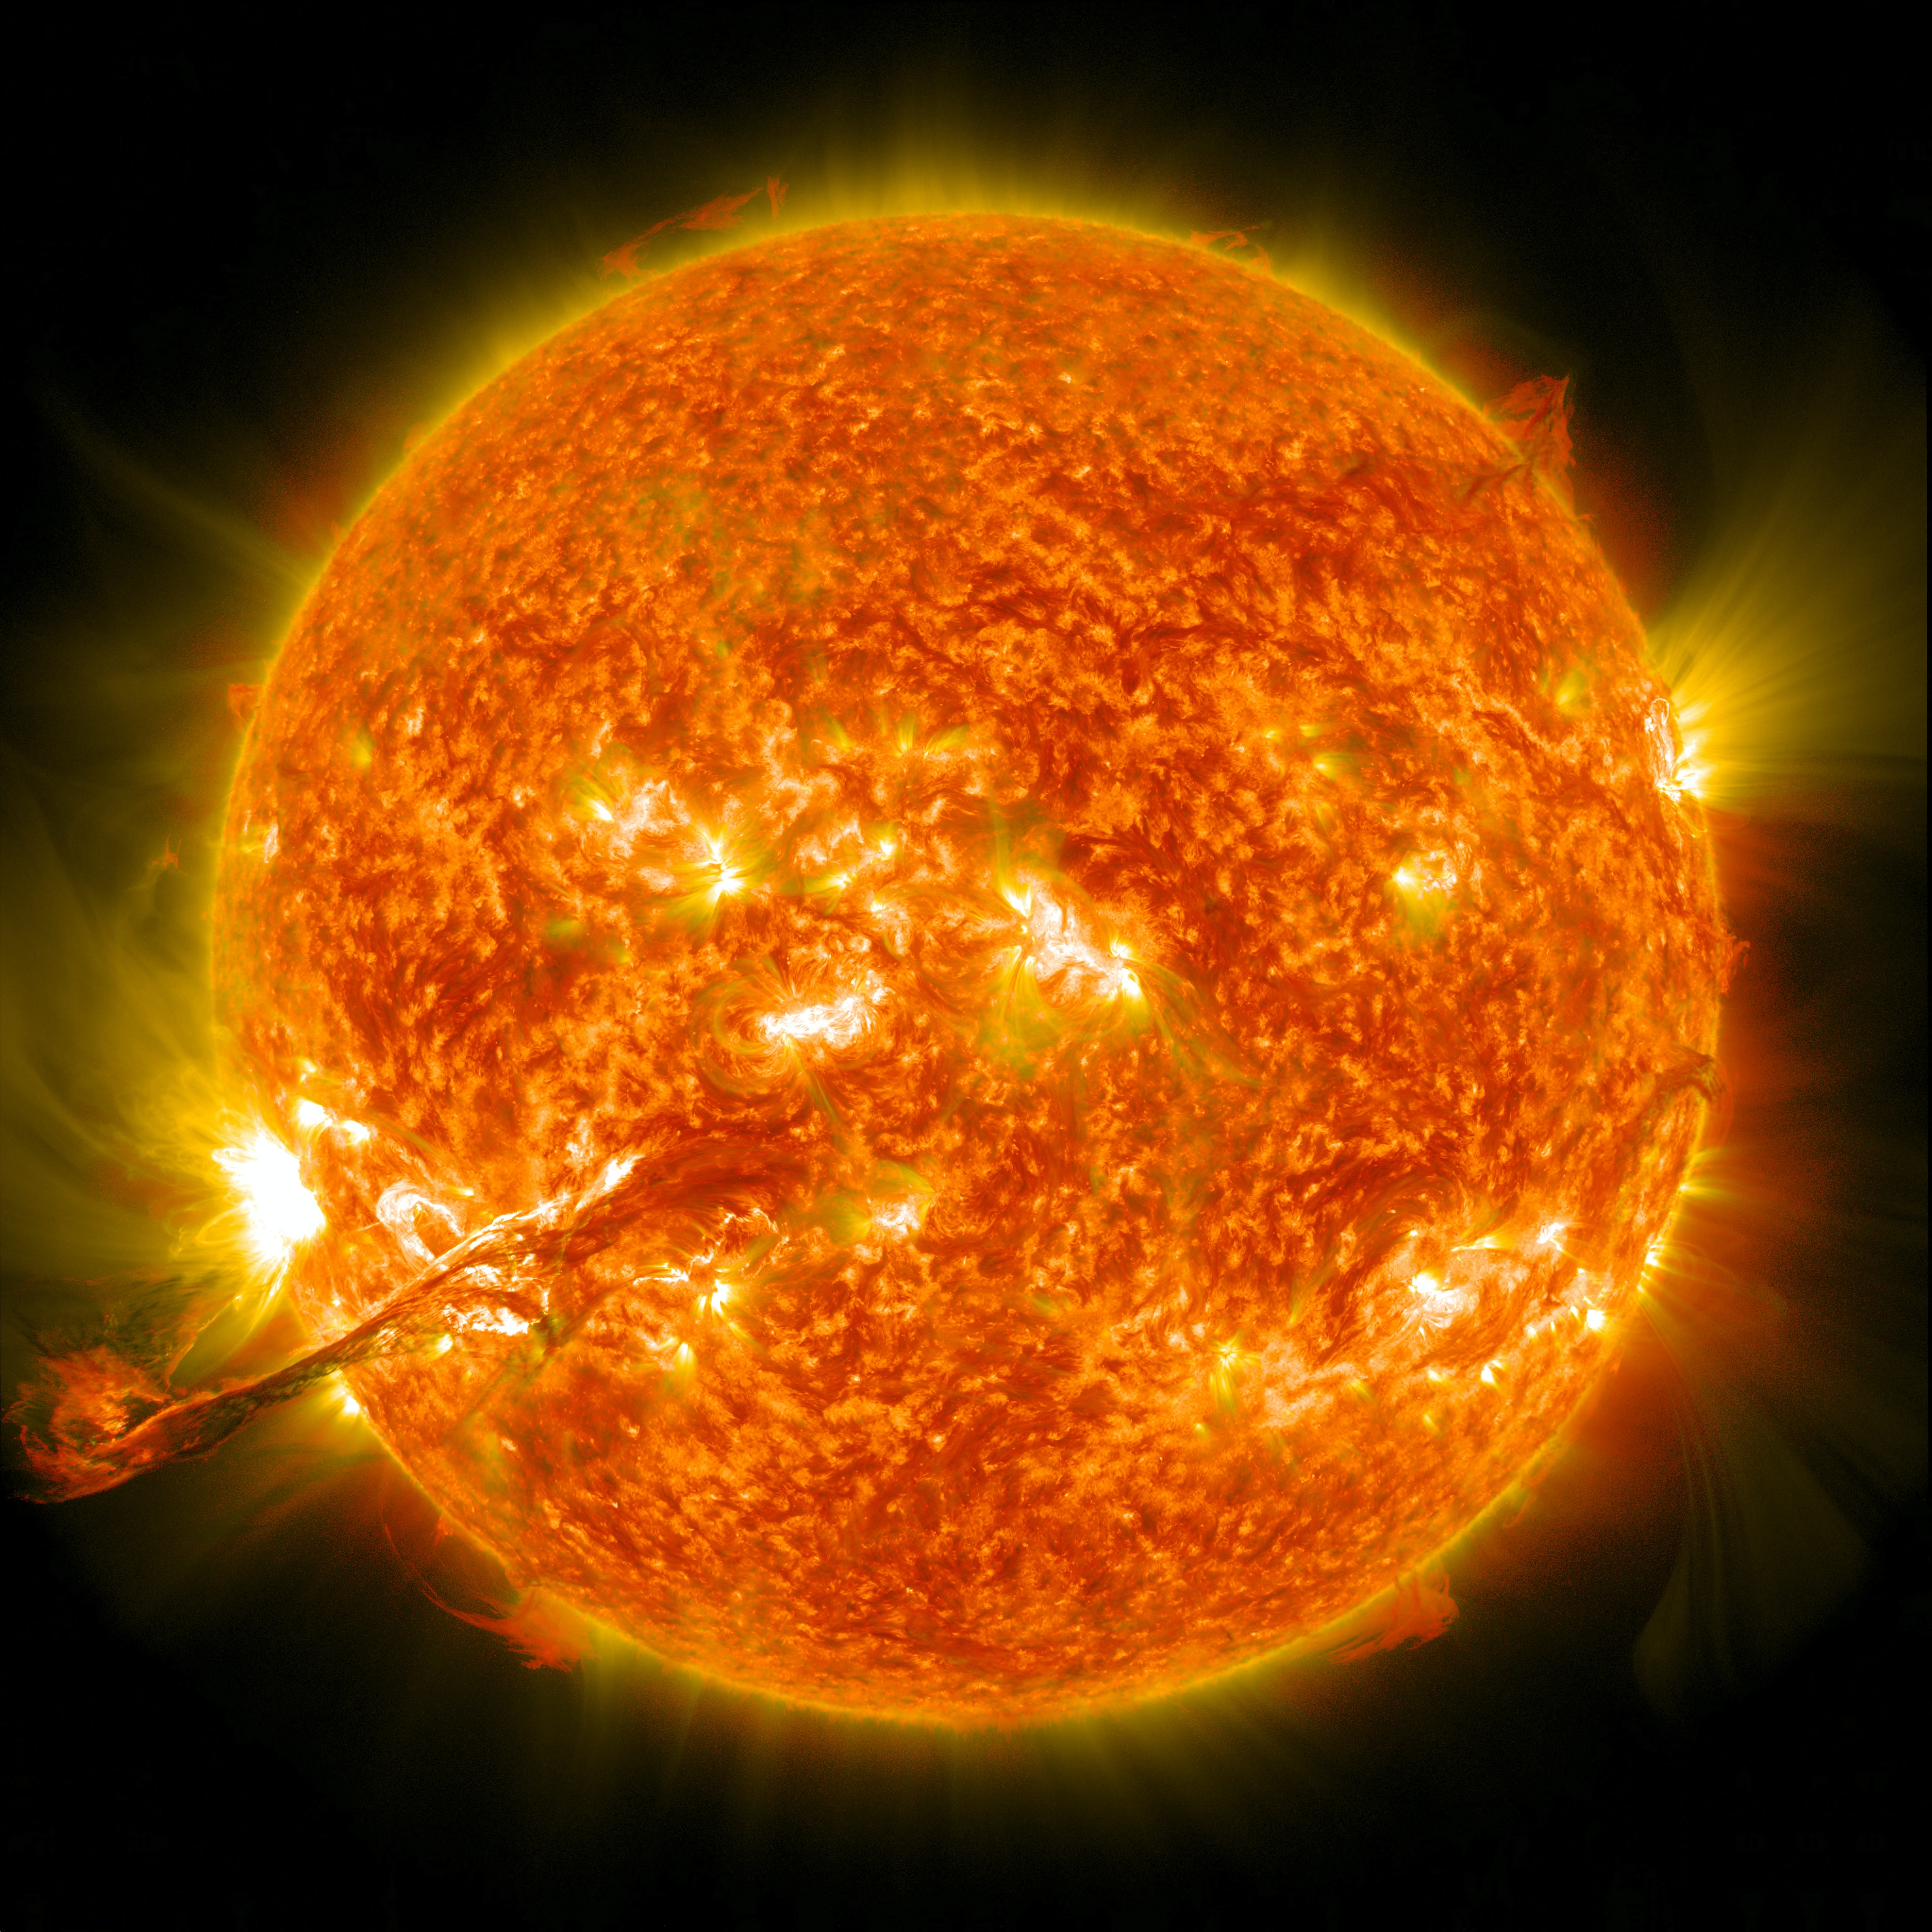
\includegraphics[width=.31\linewidth]{unsplash/nasa-cme-unsplash.jpg}%
        }%
        \visible<4>{
            % \copyrightbox[r]{
            %     % \includemovie{1cm}{1cm}{nstx/nstx.gif}
            %     \movie[
            %     height=.45\linewidth,
            %     width=.3\linewidth,
            %     autostart,
            %     loop
            %     ]{}{nstx/nstx.gif}
            % }
            % {\tiny\textbf{NSTX GPI Library} (2010 data)}
            \copyrightbox[r]{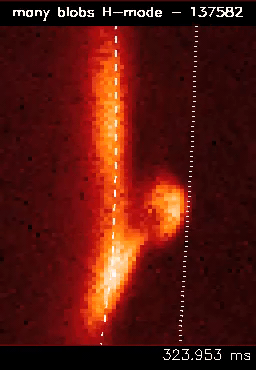
\includegraphics[width=.31\linewidth]{blobs/blobpng_284.png}}
            {\tiny\textbf{NSTX GPI Library} (2010 data)}
        }
    \end{figure}

    \note<+>{
        \begin{itemize}
            \item As our model we use the filtered Poisson process, which is a
                phenemenological model describing intermittent processes
            \item This means the model does not in itself give any insight in some
                specific physical process, but it is a powerful tool that can be used
                to investigate phenomena that show intermittency
        \end{itemize}
    }
    \note<+>{
        \begin{itemize}
            \item One example is temperature response to volcanoes which we will look at in this presentation
        \end{itemize}
    }
    \note<+>{
        \begin{itemize}
            \item Such processes can also be found in solar flares
        \end{itemize}
    }
    \note<+>{
        \begin{itemize}
            \item Or as Sajidah showed in her talk, fluctuations in fusion plasma devices
        \end{itemize}
    }

\end{frame}

\begin{frame}{Filtered Poisson process --- Definition}

    The underlying phenemenological model:

    \begin{columns}
        \begin{column}{.51\linewidth}
            \begin{equation}\label{eq:fpp_sum}
                % \alt<2>{T_K(t)}{\Phi_K(t)}=\sum_{k=1}^{\alt<2>{K}{K(T)}} A_k \phi\left(\frac{t-t_k}{\tau_\mathrm{d}}\right)
                T_K(t)=\sum_{k=1}^{K} \alt<2>{\alert{A_k}}{A_k} \phi
                \left(\frac{t-\alt<3>{\alert{t_k}}{t_k}}{\alt<4>{\alert{\tau_\mathrm{d}}}{\tau_\mathrm{d}}}\right)
            \end{equation}
            \visible<5->{\vspace{-3mm}
                \begin{equation*}
                    \downarrow
                \end{equation*}
                \begin{equation}\label{eq:fpp_convolve}
                    % \alt<2>{T_K(t)}{\Phi_K(t)}=[\phi * f_K]\left(\frac{t}{\tau_\mathrm{d}}\right)
                    T_K(t)=[\phi * f_K]\left(\frac{t}{\tau_\mathrm{d}}\right)
                \end{equation}
            }
        \end{column}
        \begin{column}{.65\linewidth}
            \begin{figure}
                \centering
                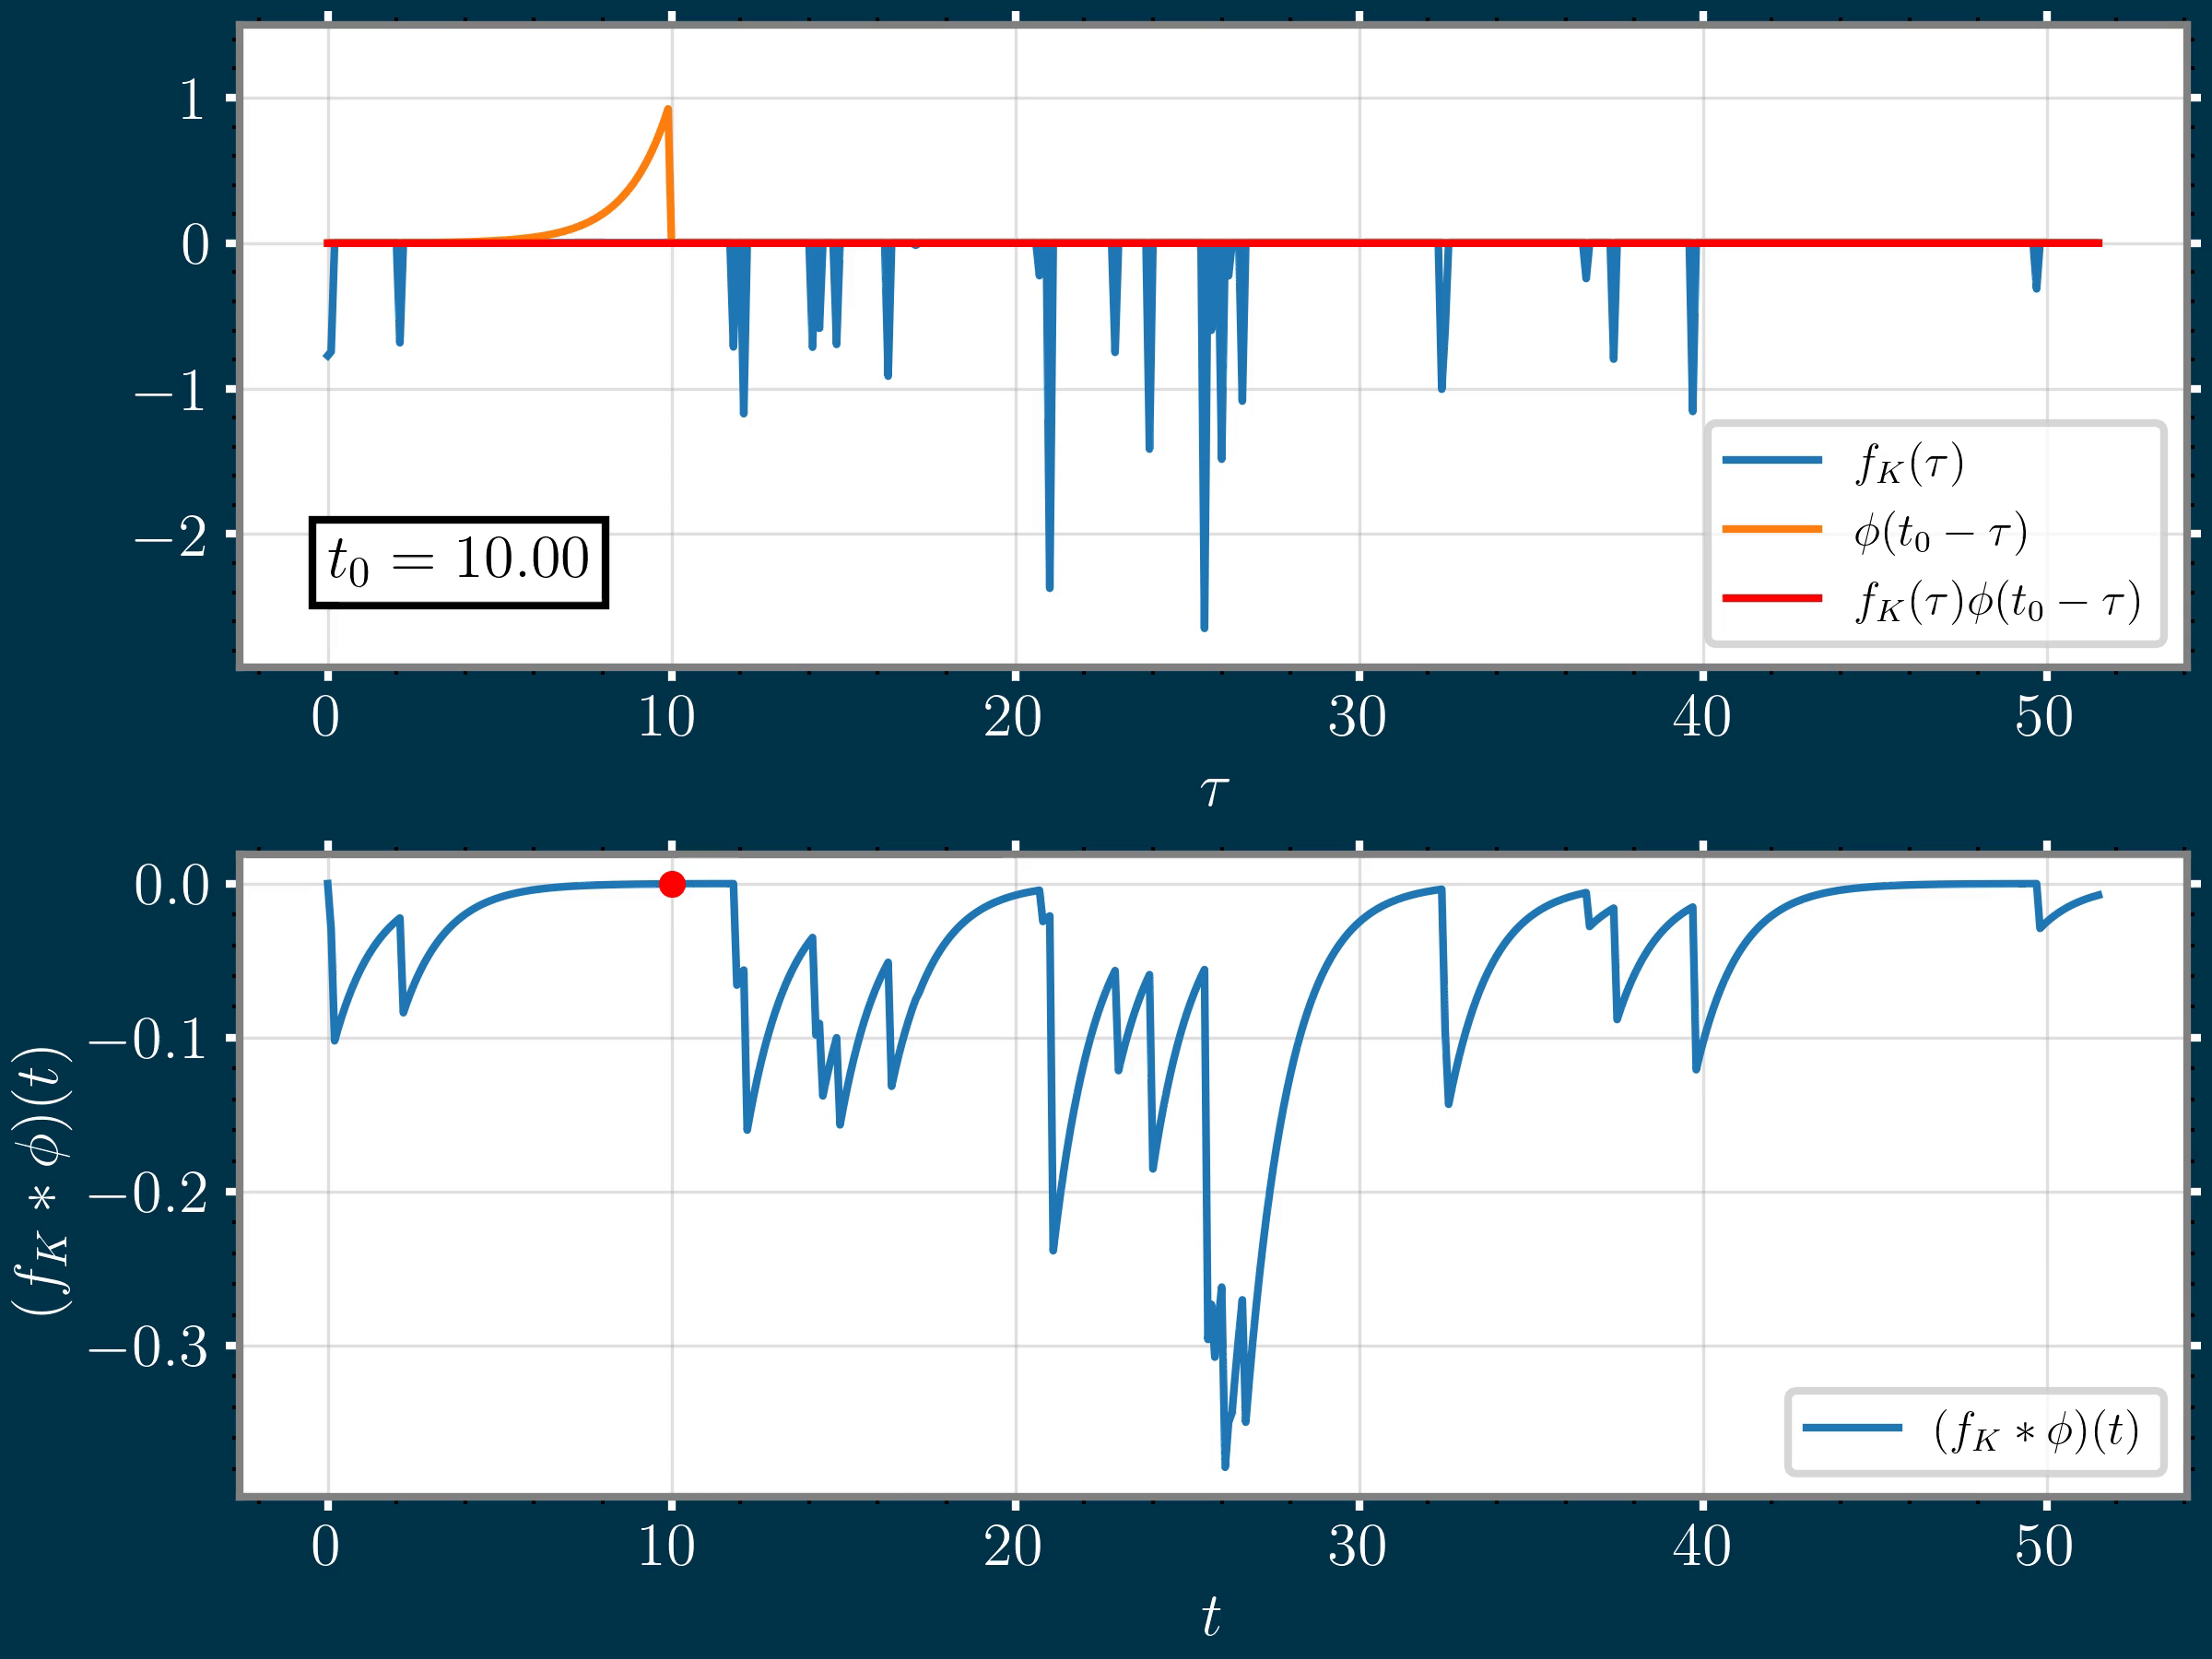
\includegraphics[width=.8\linewidth]{anim.png}
            \end{figure}
        \end{column}
    \end{columns}

    \note<+>{
        \begin{itemize}
            \item So let us look more closely at the FPP
            \item Superpos of individual volcanic events\ldots
        \end{itemize}
    }
    \note<+>{\ldots where each pulse has some amplitude \(A_k\)\ldots}
    \note<+>{\ldots they arrive according to a Poisson process at times \(t_k\)\ldots}
    \note<+>{\ldots and their duration is constant, given as \(\tau_\mathrm{d}\)}
    \note<+>{
        \begin{itemize}
            \item Can be written up as a convolution equation, where a common pulse
                shape is convolved with a forcing, which is also a sum of individual
                pulses, interpreted as volcanic eruptions
            \item We se in the animation how the convolution is done
            \item This assumes knowledge about the response function and the
                forcing, which gives you temperature as the output, so we need a method
                of turning it around
        \end{itemize}
    }

\end{frame}

% \begin{frame}{Simple raycasting animation}
%     \animategraphics[controls,loop,autoplay]{1}{conv-}{0}{16}
% \end{frame}

\begin{frame}{Filtered Poisson process --- Definition}

    The underlying phenemenological model:

    \begin{columns}
        \begin{column}{.51\linewidth}
            % \begin{equation}\label{eq:fpp_sum}
            %   % \alt<2>{T_K(t)}{\Phi_K(t)}=\sum_{k=1}^{\alt<2>{K}{K(T)}} A_k \phi\left(\frac{t-t_k}{\tau_\mathrm{d}}\right)
            %   T_K(t)=\sum_{k=1}^{K} A_k \phi\left(\frac{t-t_k}{\tau_\mathrm{d}}\right)
            % \end{equation}
            % \begin{equation*}
            %   \downarrow
            % \end{equation*}
            \begin{equation}\tag{\ref{eq:fpp_convolve}}
                % \alt<2>{T_K(t)}{\Phi_K(t)}=[\phi * f_K]\left(\frac{t}{\tau_\mathrm{d}}\right)
                T_K(t)=[\phi * f_K]\left(\frac{t}{\tau_\mathrm{d}}\right)
            \end{equation}
        \end{column}
        \begin{column}{.65\linewidth}
            \begin{center}
                % \animategraphics[autoplay,loop,width=.8\linewidth]{10}{gif/conv-}{0}{16}
                % 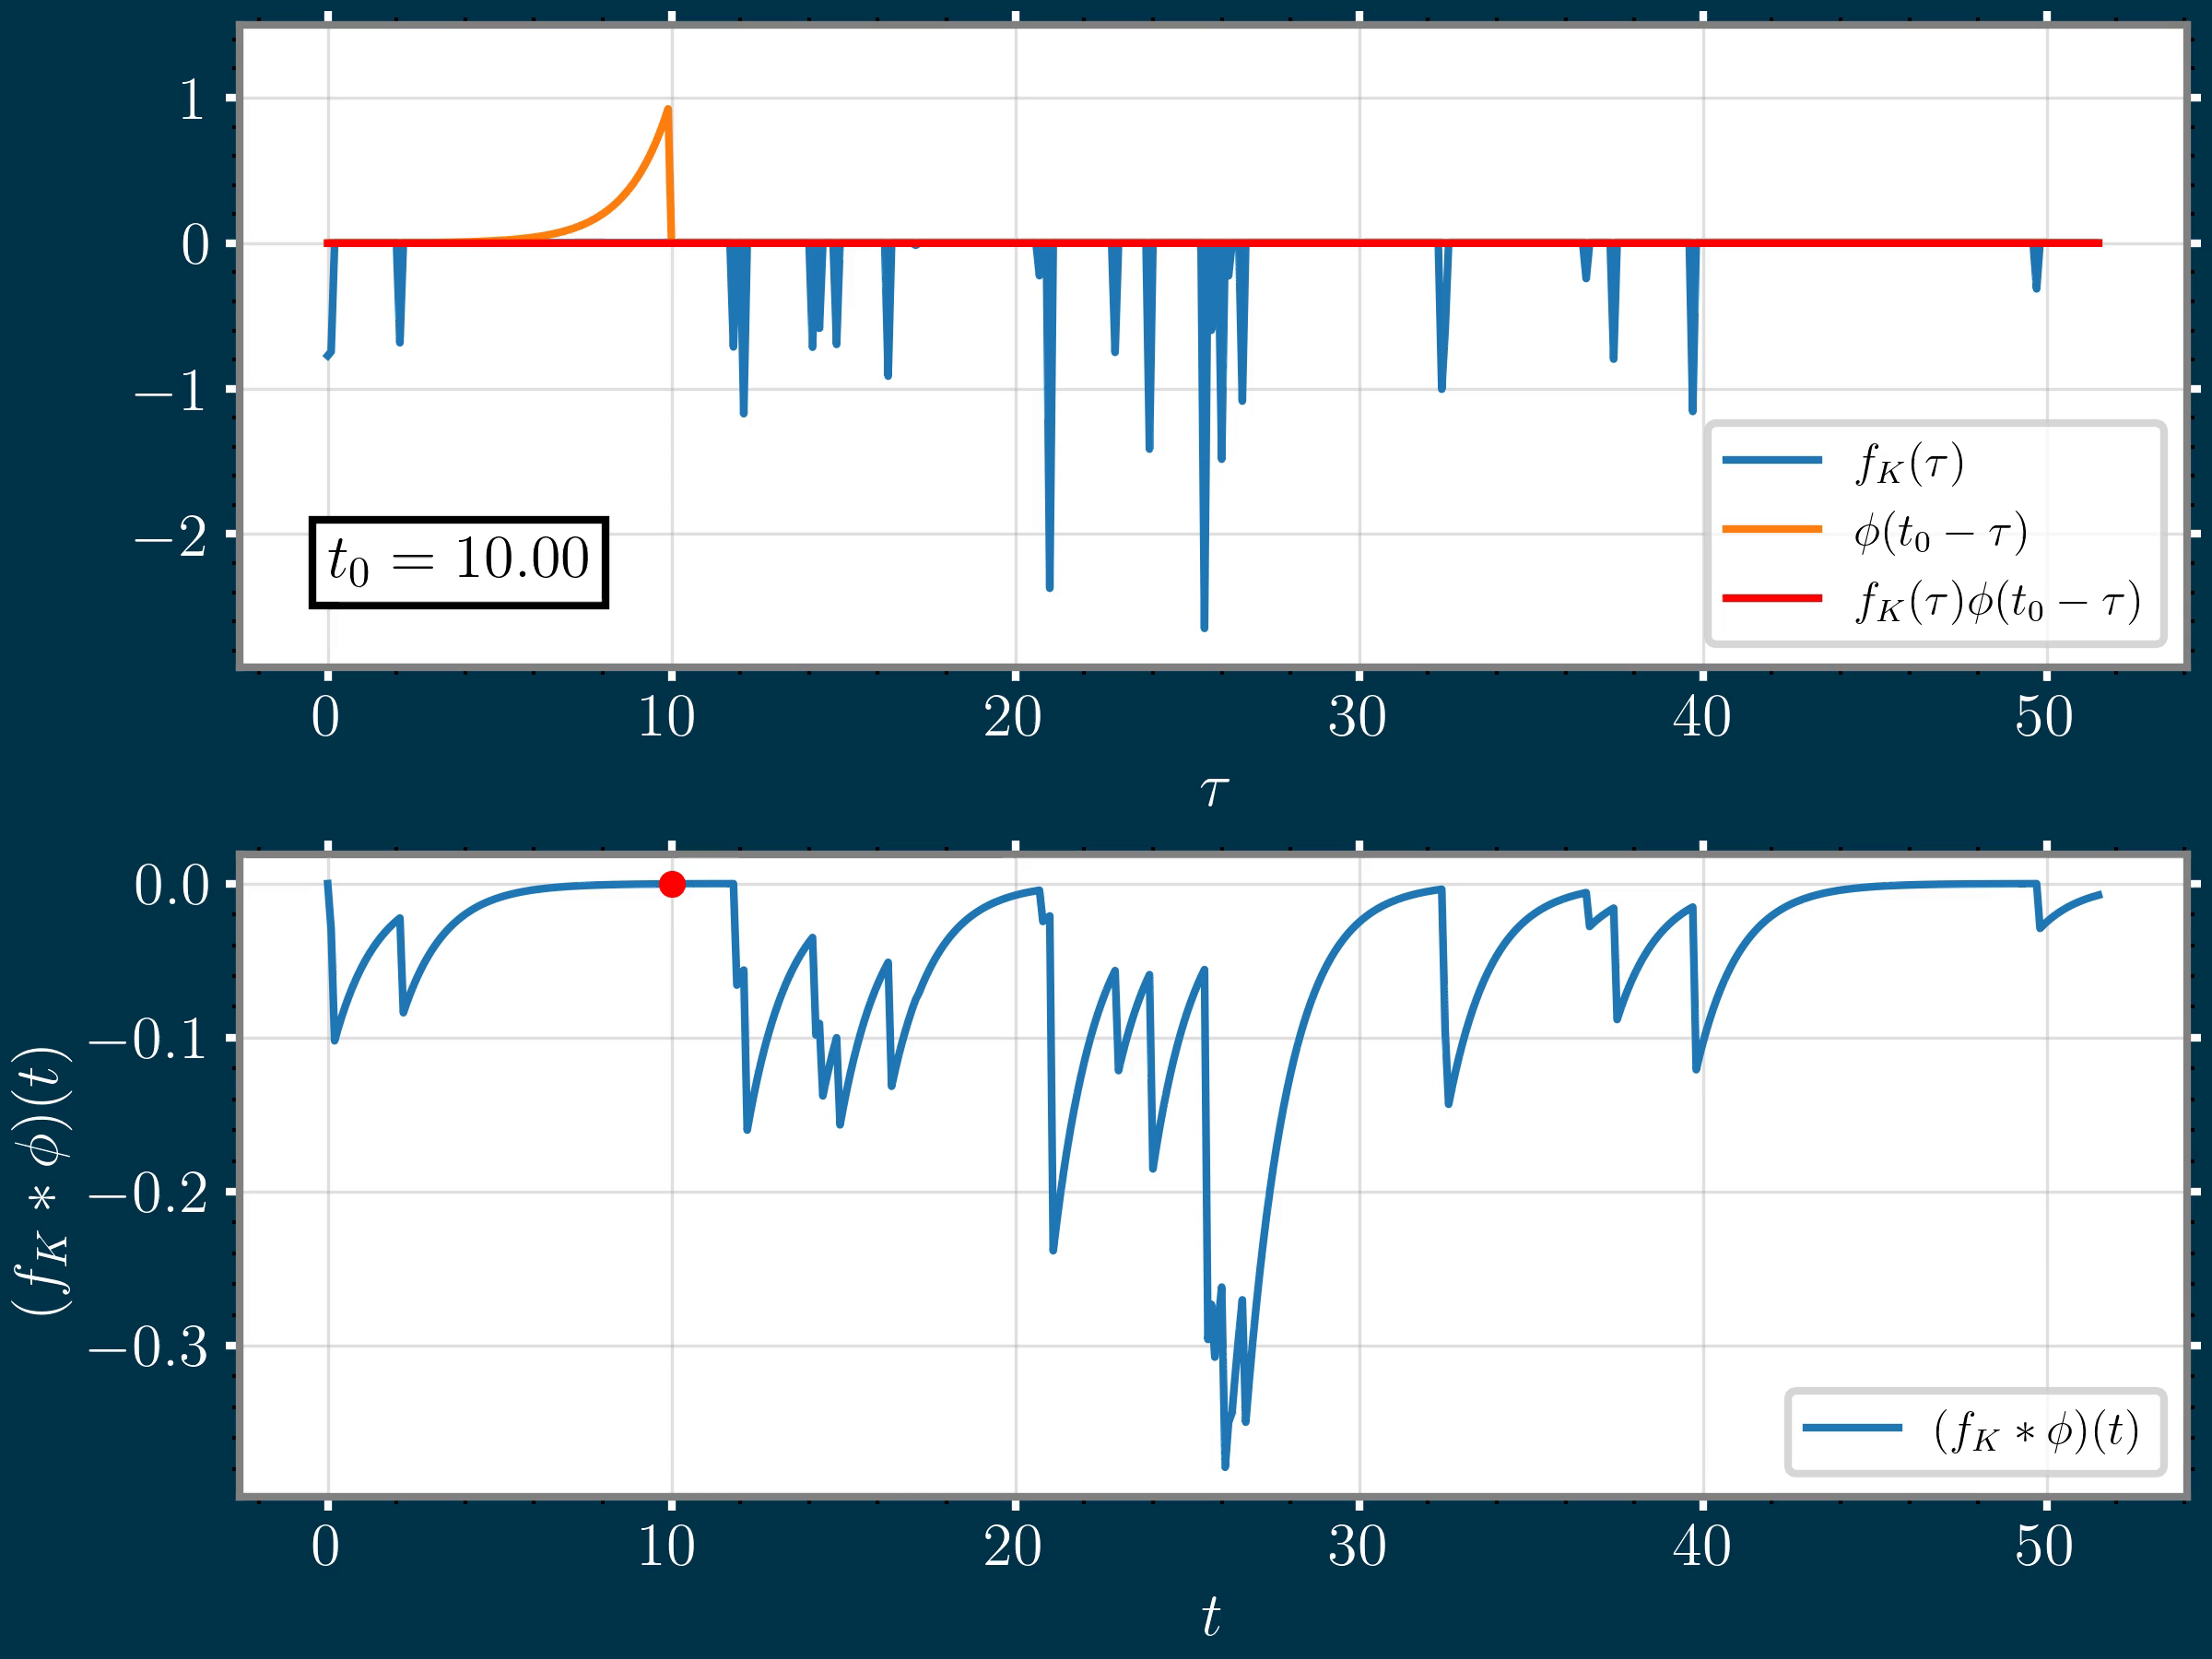
\includegraphics[width=.8\linewidth]{anim.png}
                \movie[
                height=.6\linewidth,
                width=.8\linewidth,
                autostart,
                loop
                ]{}{animation.mp4}
            \end{center}
        \end{column}
    \end{columns}

    \note<+>{
        \begin{itemize}
            \item So let us look more closely at the FPP
            \item Superpos of pulses with amplitudes \(A_k\), arrive according to a
                Poisson process at times \(t_k\) and their duration is constant:
                \(\tau_\mathrm{d}\)
            \item Can be written up as a convolution equation, where a common pulse
                shape is convolved with a forcing, which is also a sum of individual
                pulses, interpreted as volcanic eruptions
            \item We see in the animation how the convolution is done
            \item This assumes knowledge about the response function and the
                forcing, which gives you temperature as the output, so we need a method
                of turning it around
        \end{itemize}
    }

\end{frame}
% \begin{frame}
%   \frametitle{Filtered Poisson process --- Definition}

%   The underlying phenemenological model:

%   \begin{columns}
%     \begin{column}{.51\linewidth}
%       \begin{overprint}
%       \onslide<1>
%         \begin{equation}\label{eq:fpp_sum}
%           % \alt<2>{T_K(t)}{\Phi_K(t)}=\sum_{k=1}^{\alt<2>{K}{K(T)}} A_k \phi\left(\frac{t-t_k}{\tau_\mathrm{d}}\right)
%           \Phi_K(t)=\sum_{k=1}^{K(T)} A_k \phi\left(\frac{t-t_k}{\tau_\mathrm{d}}\right)
%         \end{equation}
%         \begin{equation*}
%           \downarrow
%         \end{equation*}
%         \begin{equation}\label{eq:fpp_convolve}
%           % \alt<2>{T_K(t)}{\Phi_K(t)}=[\phi * f_K]\left(\frac{t}{\tau_\mathrm{d}}\right)
%           \Phi_K(t)=[\phi * f_K]\left(\frac{t}{\tau_\mathrm{d}}\right)
%         \end{equation}
%       \onslide<2>
%       \begin{equation}\tag{\ref{eq:fpp_sum}}
%           % \alt<2>{T_K(t)}{\Phi_K(t)}=\sum_{k=1}^{\alt<2>{K}{K(T)}} A_k \phi\left(\frac{t-t_k}{\tau_\mathrm{d}}\right)
%           T_K(t)=\sum_{k=1}^{K} A_k \phi\left(\frac{t-t_k}{\tau_\mathrm{d}}\right)
%         \end{equation}
%         \begin{equation*}
%           \downarrow
%         \end{equation*}
%         \begin{equation}\tag{\ref{eq:fpp_convolve}}
%           % \alt<2>{T_K(t)}{\Phi_K(t)}=[\phi * f_K]\left(\frac{t}{\tau_\mathrm{d}}\right)
%           T_K(t)=[\phi * f_K]\left(\frac{t}{\tau_\mathrm{d}}\right)
%         \end{equation}
%       \end{overprint}
%     \end{column}
%     \begin{column}{.65\linewidth}
%       \begin{center}
%         \movie[
%           height=.6\linewidth,
%           width=.8\linewidth,
%           autostart,
%           loop
%           ]{}{animation.mp4}
%       \end{center}
%       % \begin{figure}
%       %   \centering
%       %   \animategraphics[autoplay,loop,width=\linewidth]{10}{../figures/deconvolution_anim/deconvolution_}{0}{52}
%       % \end{figure}
%     \end{column}
%   \end{columns}

% \end{frame}

% \begin{frame}
%   \frametitle{Filtered Poisson process --- Definition}

%   \begin{equation}\tag{\ref{eq:fpp_convolve}}
%     T_K(t)=[\phi * f_K]\left(\frac{t}{\tau_\mathrm{d}}\right)
%   \end{equation}

%   Given:
%   \begin{itemize}
%     \item \(\tau_\mathrm{d}\) is constant
%     \item \(f_K\) is a train of delta pulses:
%       \begin{equation}
%         f_K(t)=\sum_{k=1}^{K} A_k\delta\left(\frac{t-t_k}{\tau_\mathrm{d}}\right)
%       \end{equation}
%   \end{itemize}

% \end{frame}

\subsection{Deconvolution}

\begin{frame}{Richardson-Lucy deconvolution}

    An iterative process: \cite{Lucy1974,1972richardson,benvenuto2009}
    \begin{equation}\label{eq:deconvolution}
        \phi^{(n+1)}=\phi^{(n)} \frac{(T_K-\langle T_K\rangle)*\hat{f}_K+b}{\phi^{(n)}*f_K*\hat{f}_K+b}
    \end{equation}

    \note<+>{
        \begin{itemize}
            \item We write up a deconvolution equation, which is an iterative
                algorithm that can take forcing and temperature as the input, and out
                comes the response function
            \item The constant \(b\) regularises the process, ensuring positive
                definite response function
            \item Sajidah spent time discussing this algorithm and considerations
                that are important to account for
            \item It is not trivial, but we will simply apply it in this presentation
        \end{itemize}
    }

\end{frame}


\section{Method}
\subsection{Filtered Poisson process}

\begin{frame}{Filtered Poisson process --- Examples}

    The FPP model intermittent processes:\vspace{-13mm}
    \begin{figure}
        \centering
        \visible<2->{
            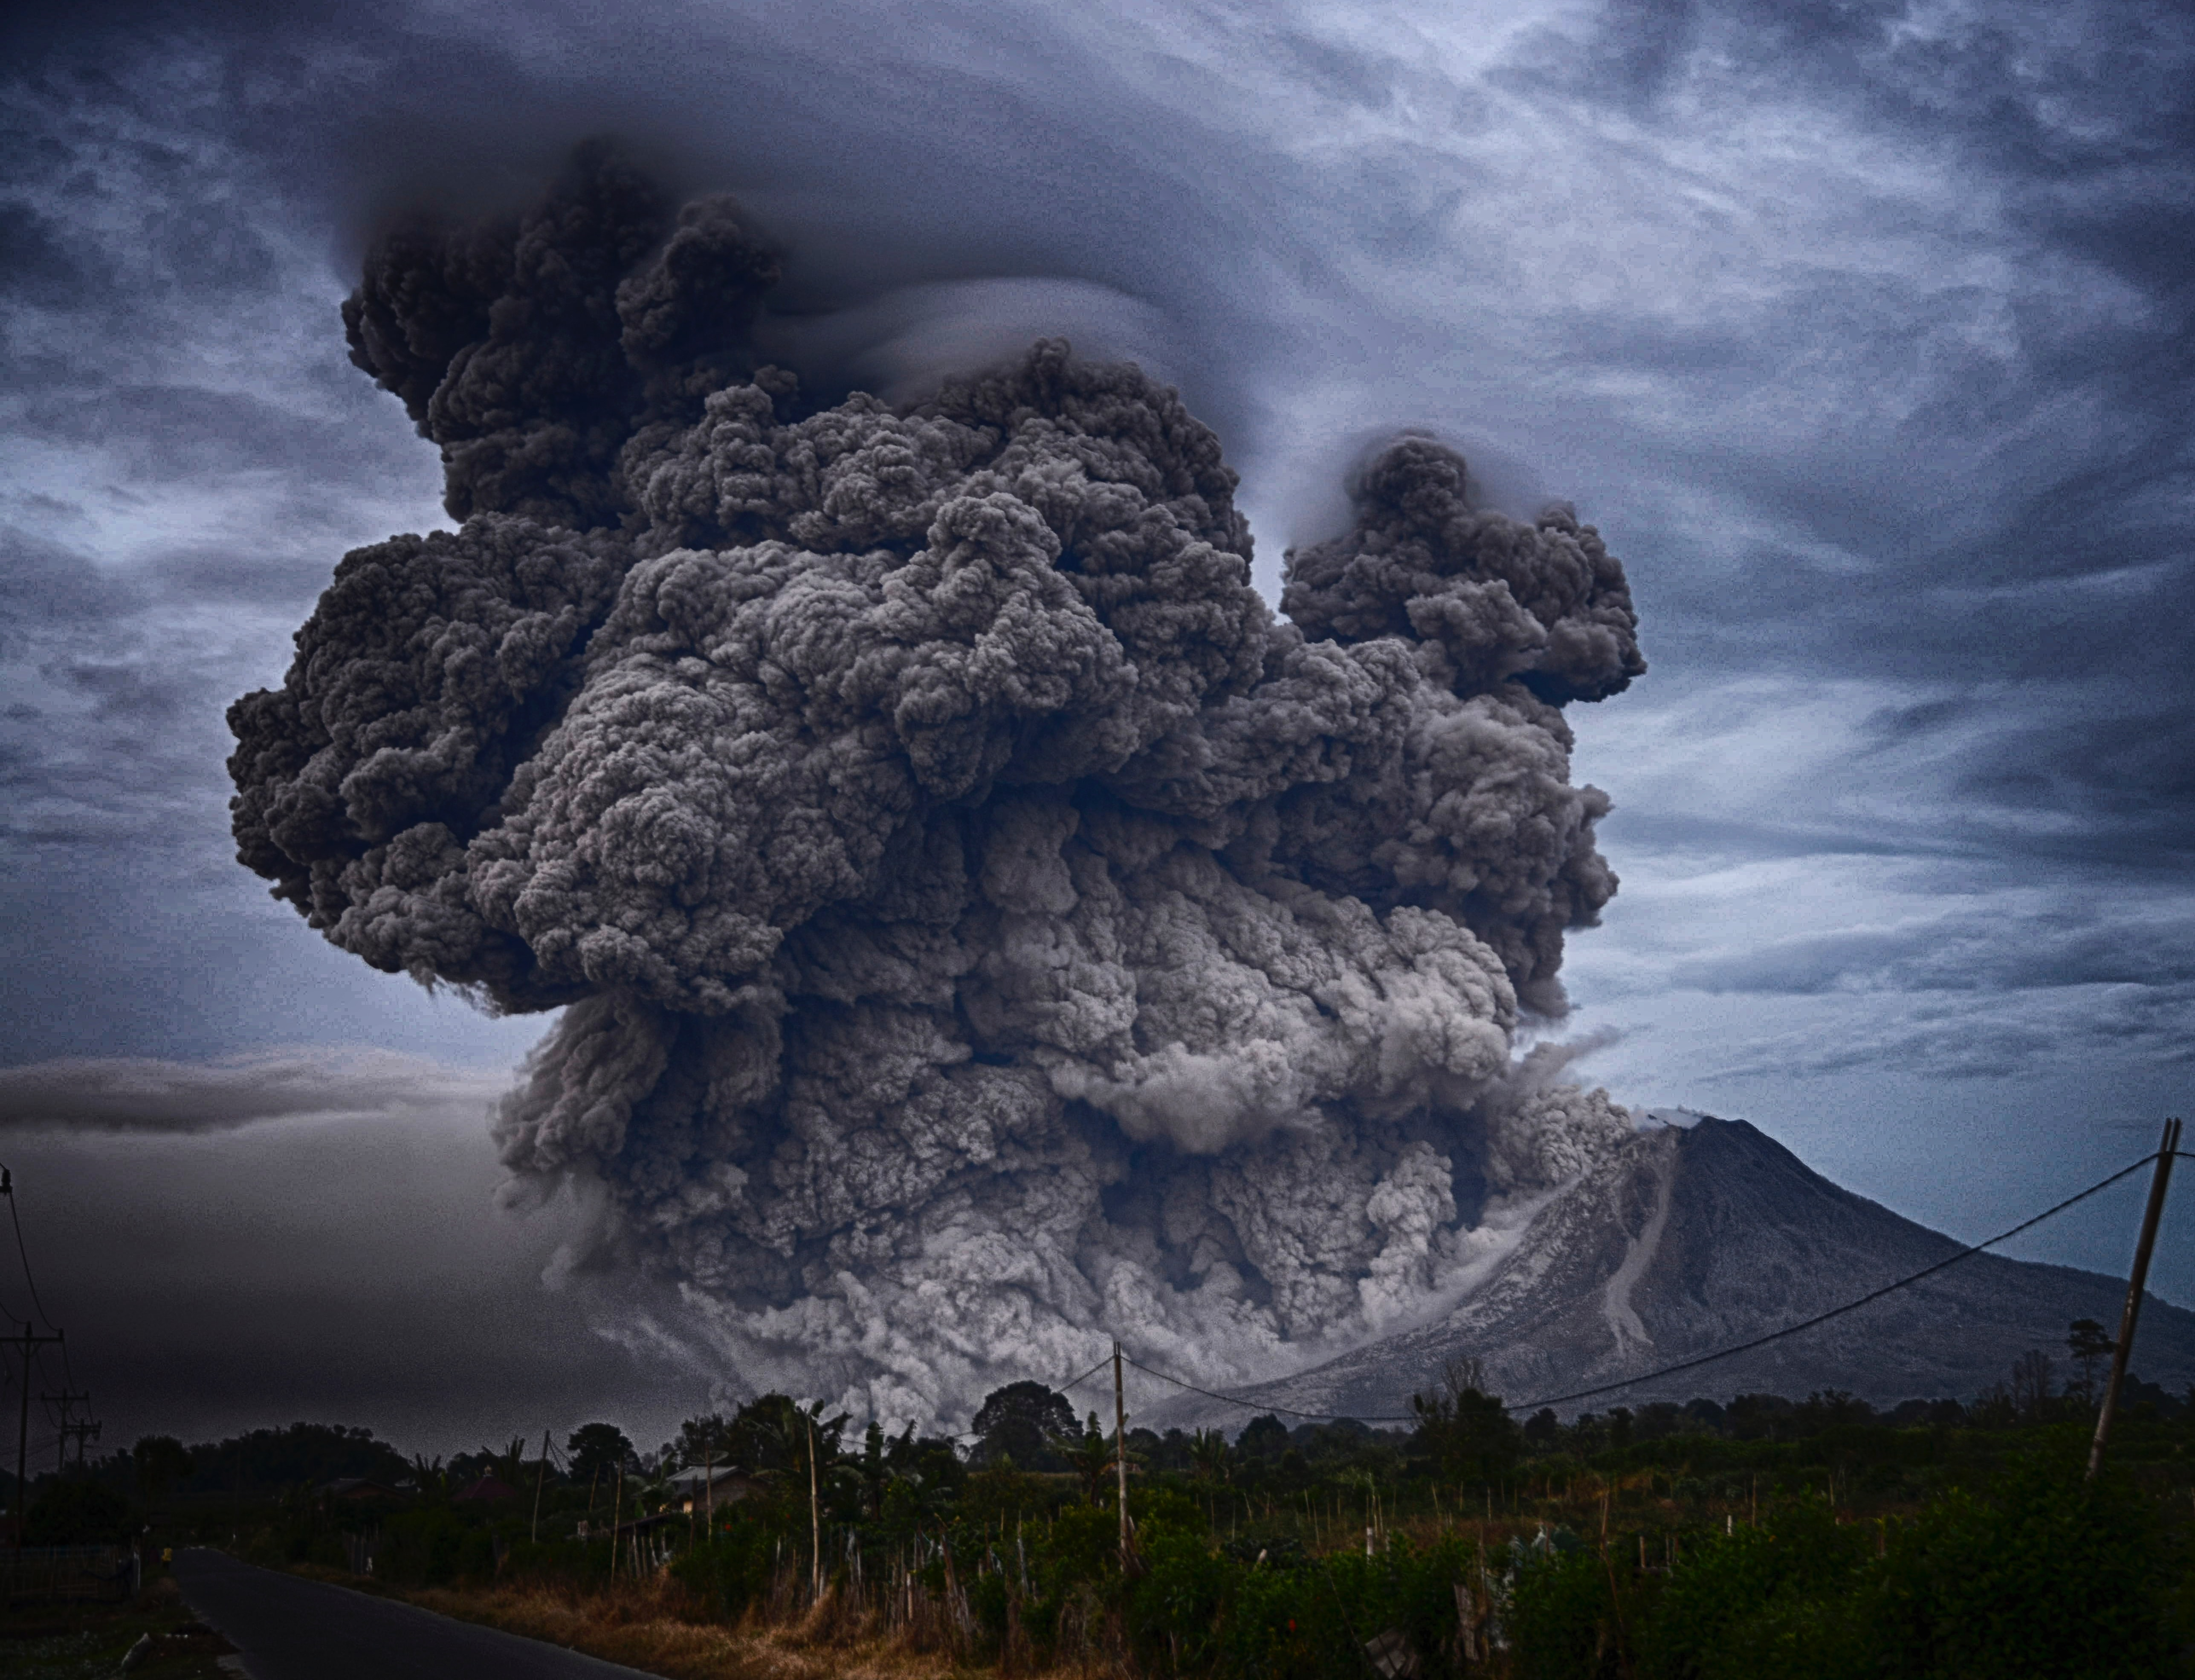
\includegraphics[width=.31\linewidth]{unsplash/volcano-unsplash.jpg}
        }
        \visible<3->{
            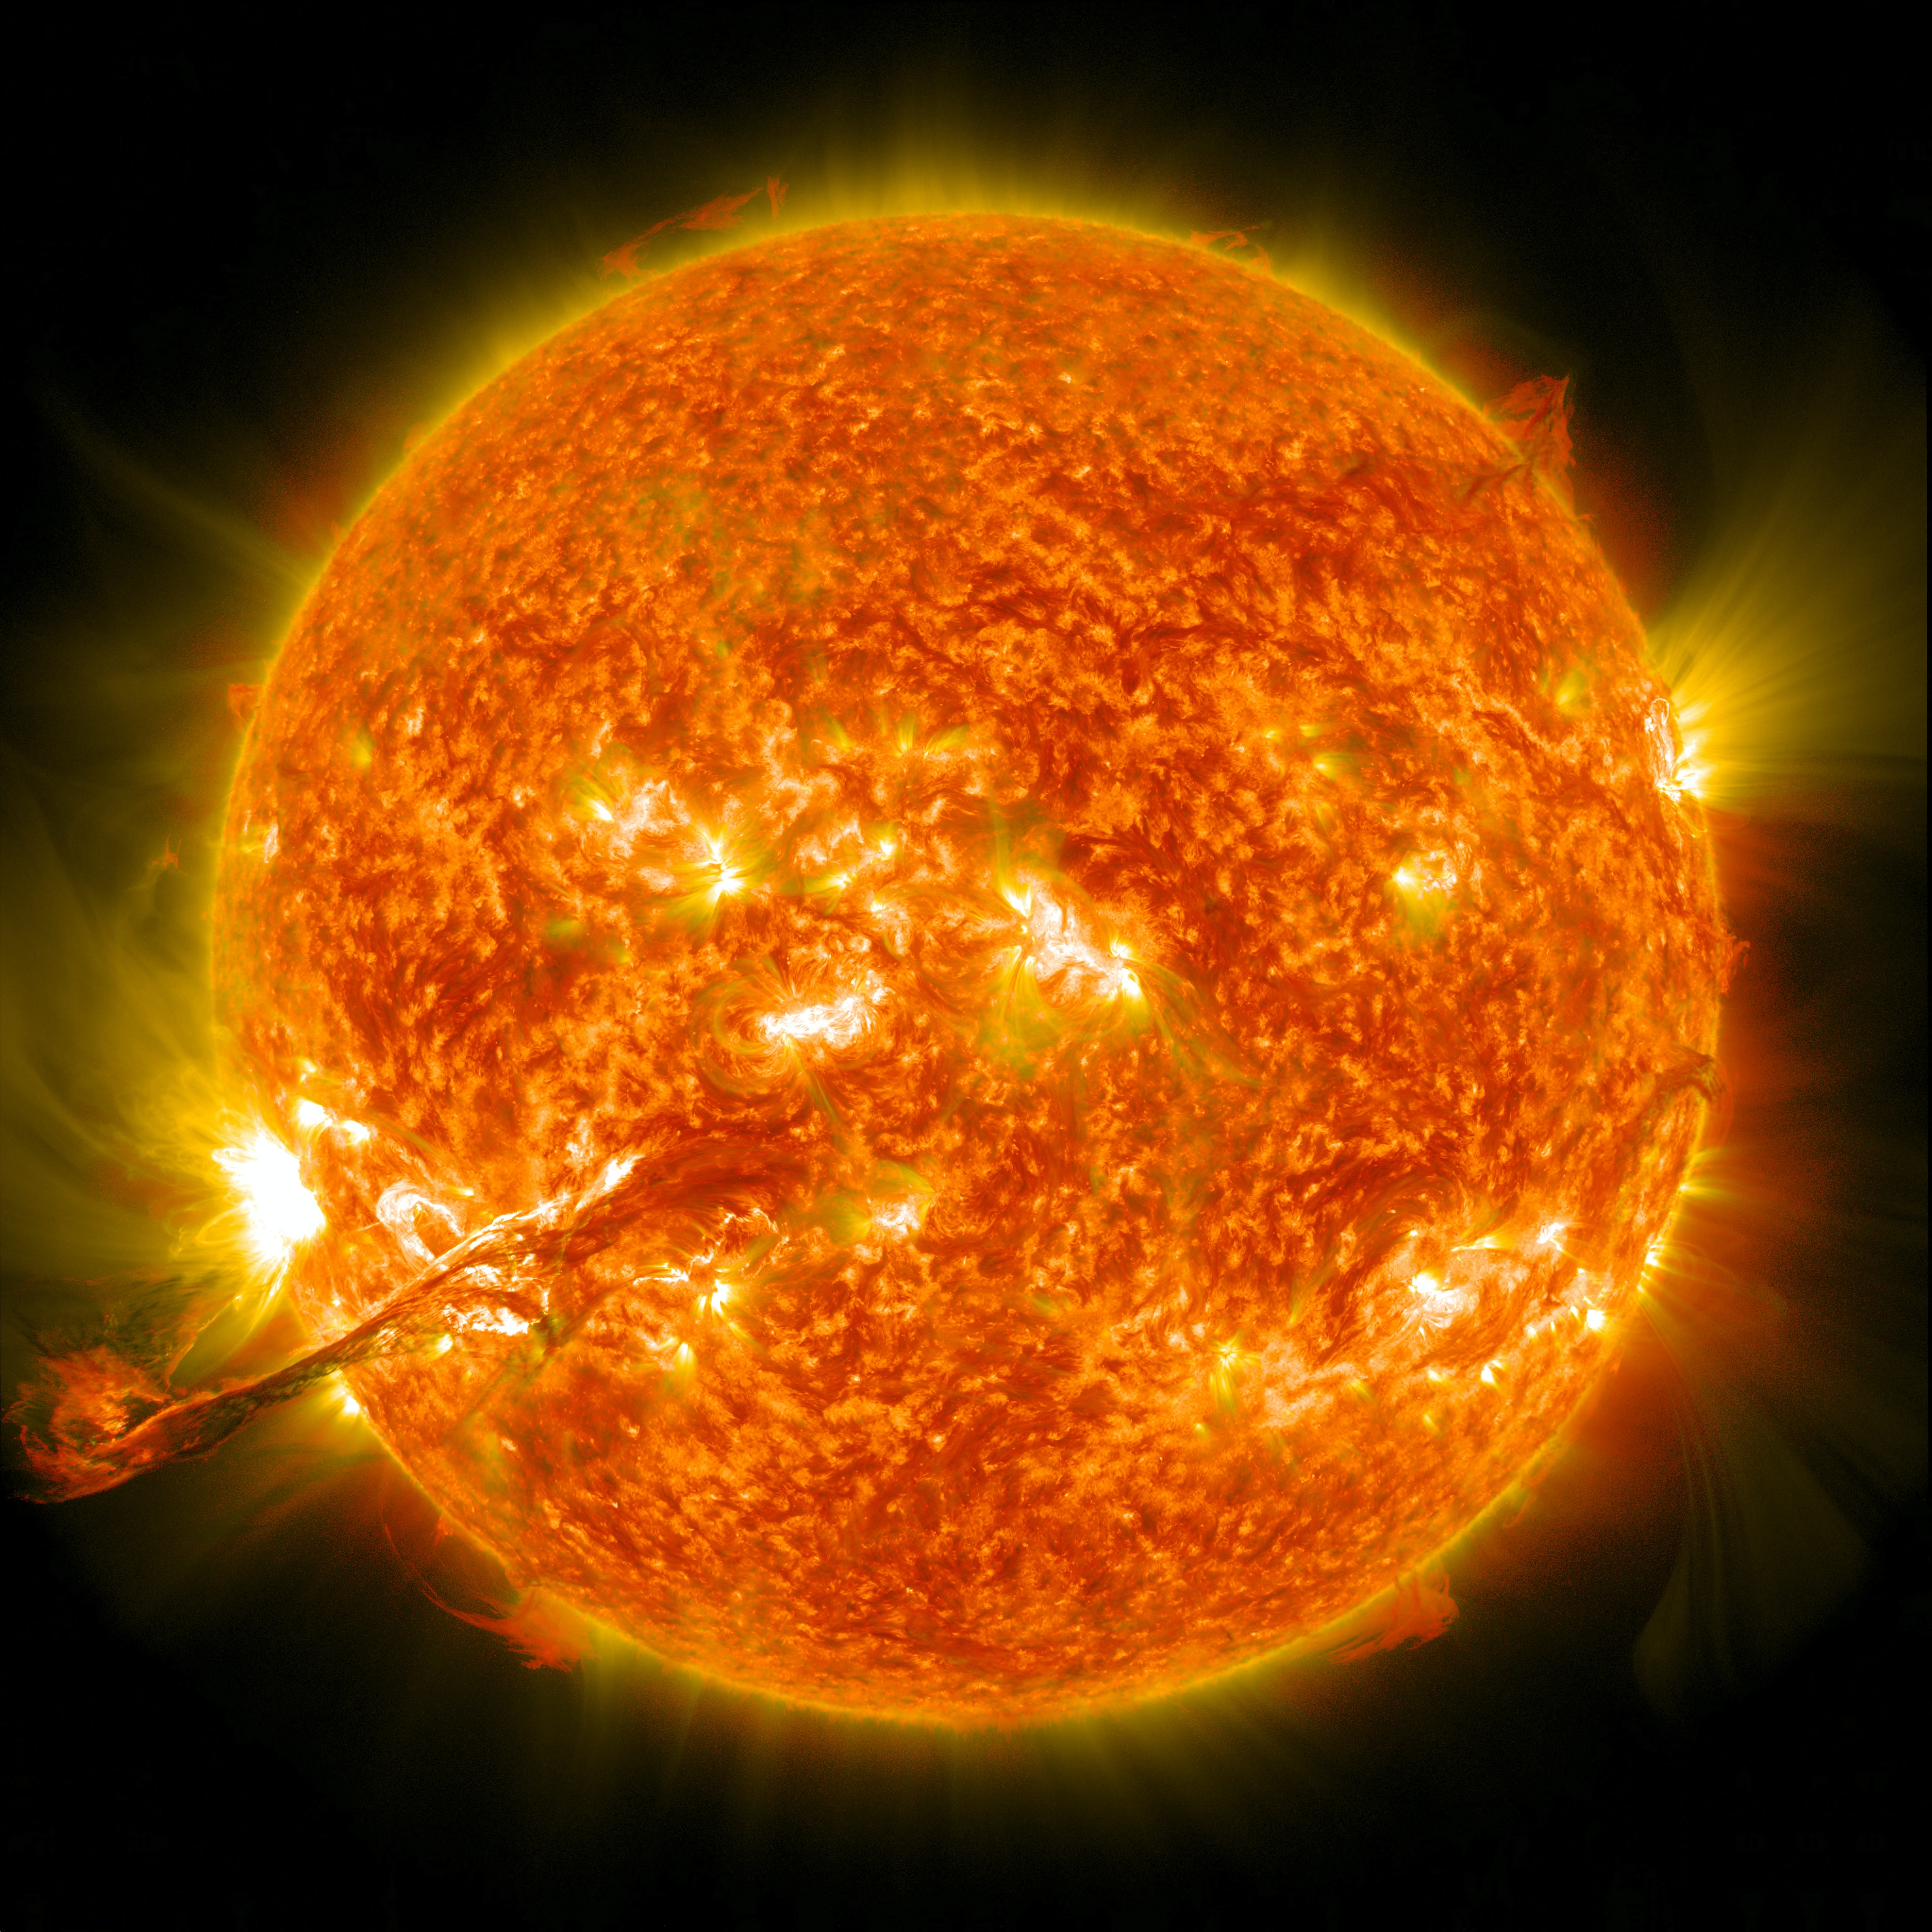
\includegraphics[width=.31\linewidth]{unsplash/nasa-cme-unsplash.jpg}%
        }%
        \visible<4>{
            % \copyrightbox[r]{
            %     % \includemovie{1cm}{1cm}{nstx/nstx.gif}
            %     \movie[
            %     height=.45\linewidth,
            %     width=.3\linewidth,
            %     autostart,
            %     loop
            %     ]{}{nstx/nstx.gif}
            % }
            % {\tiny\textbf{NSTX GPI Library} (2010 data)}
            \copyrightbox[r]{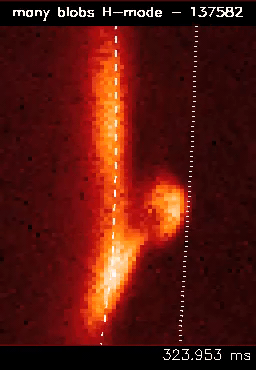
\includegraphics[width=.31\linewidth]{blobs/blobpng_284.png}}
            {\tiny\textbf{NSTX GPI Library} (2010 data)}
        }
    \end{figure}

    \note<+>{
        \begin{itemize}
            \item As our model we use the filtered Poisson process, which is a
                phenemenological model describing intermittent processes
            \item This means the model does not in itself give any insight in some
                specific physical process, but it is a powerful tool that can be used
                to investigate phenomena that show intermittency
        \end{itemize}
    }
    \note<+>{
        \begin{itemize}
            \item One example is temperature response to volcanoes which we will look at in this presentation
        \end{itemize}
    }
    \note<+>{
        \begin{itemize}
            \item Such processes can also be found in solar flares
        \end{itemize}
    }
    \note<+>{
        \begin{itemize}
            \item Or as Sajidah showed in her talk, fluctuations in fusion plasma devices
        \end{itemize}
    }

\end{frame}

\begin{frame}{Filtered Poisson process --- Definition}

    The underlying phenemenological model:

    \begin{columns}
        \begin{column}{.51\linewidth}
            \begin{equation}\label{eq:fpp_sum}
                % \alt<2>{T_K(t)}{\Phi_K(t)}=\sum_{k=1}^{\alt<2>{K}{K(T)}} A_k \phi\left(\frac{t-t_k}{\tau_\mathrm{d}}\right)
                T_K(t)=\sum_{k=1}^{K} \alt<2>{\alert{A_k}}{A_k} \phi
                \left(\frac{t-\alt<3>{\alert{t_k}}{t_k}}{\alt<4>{\alert{\tau_\mathrm{d}}}{\tau_\mathrm{d}}}\right)
            \end{equation}
            \visible<5->{\vspace{-3mm}
                \begin{equation*}
                    \downarrow
                \end{equation*}
                \begin{equation}\label{eq:fpp_convolve}
                    % \alt<2>{T_K(t)}{\Phi_K(t)}=[\phi * f_K]\left(\frac{t}{\tau_\mathrm{d}}\right)
                    T_K(t)=[\phi * f_K]\left(\frac{t}{\tau_\mathrm{d}}\right)
                \end{equation}
            }
        \end{column}
        \begin{column}{.65\linewidth}
            \begin{figure}
                \centering
                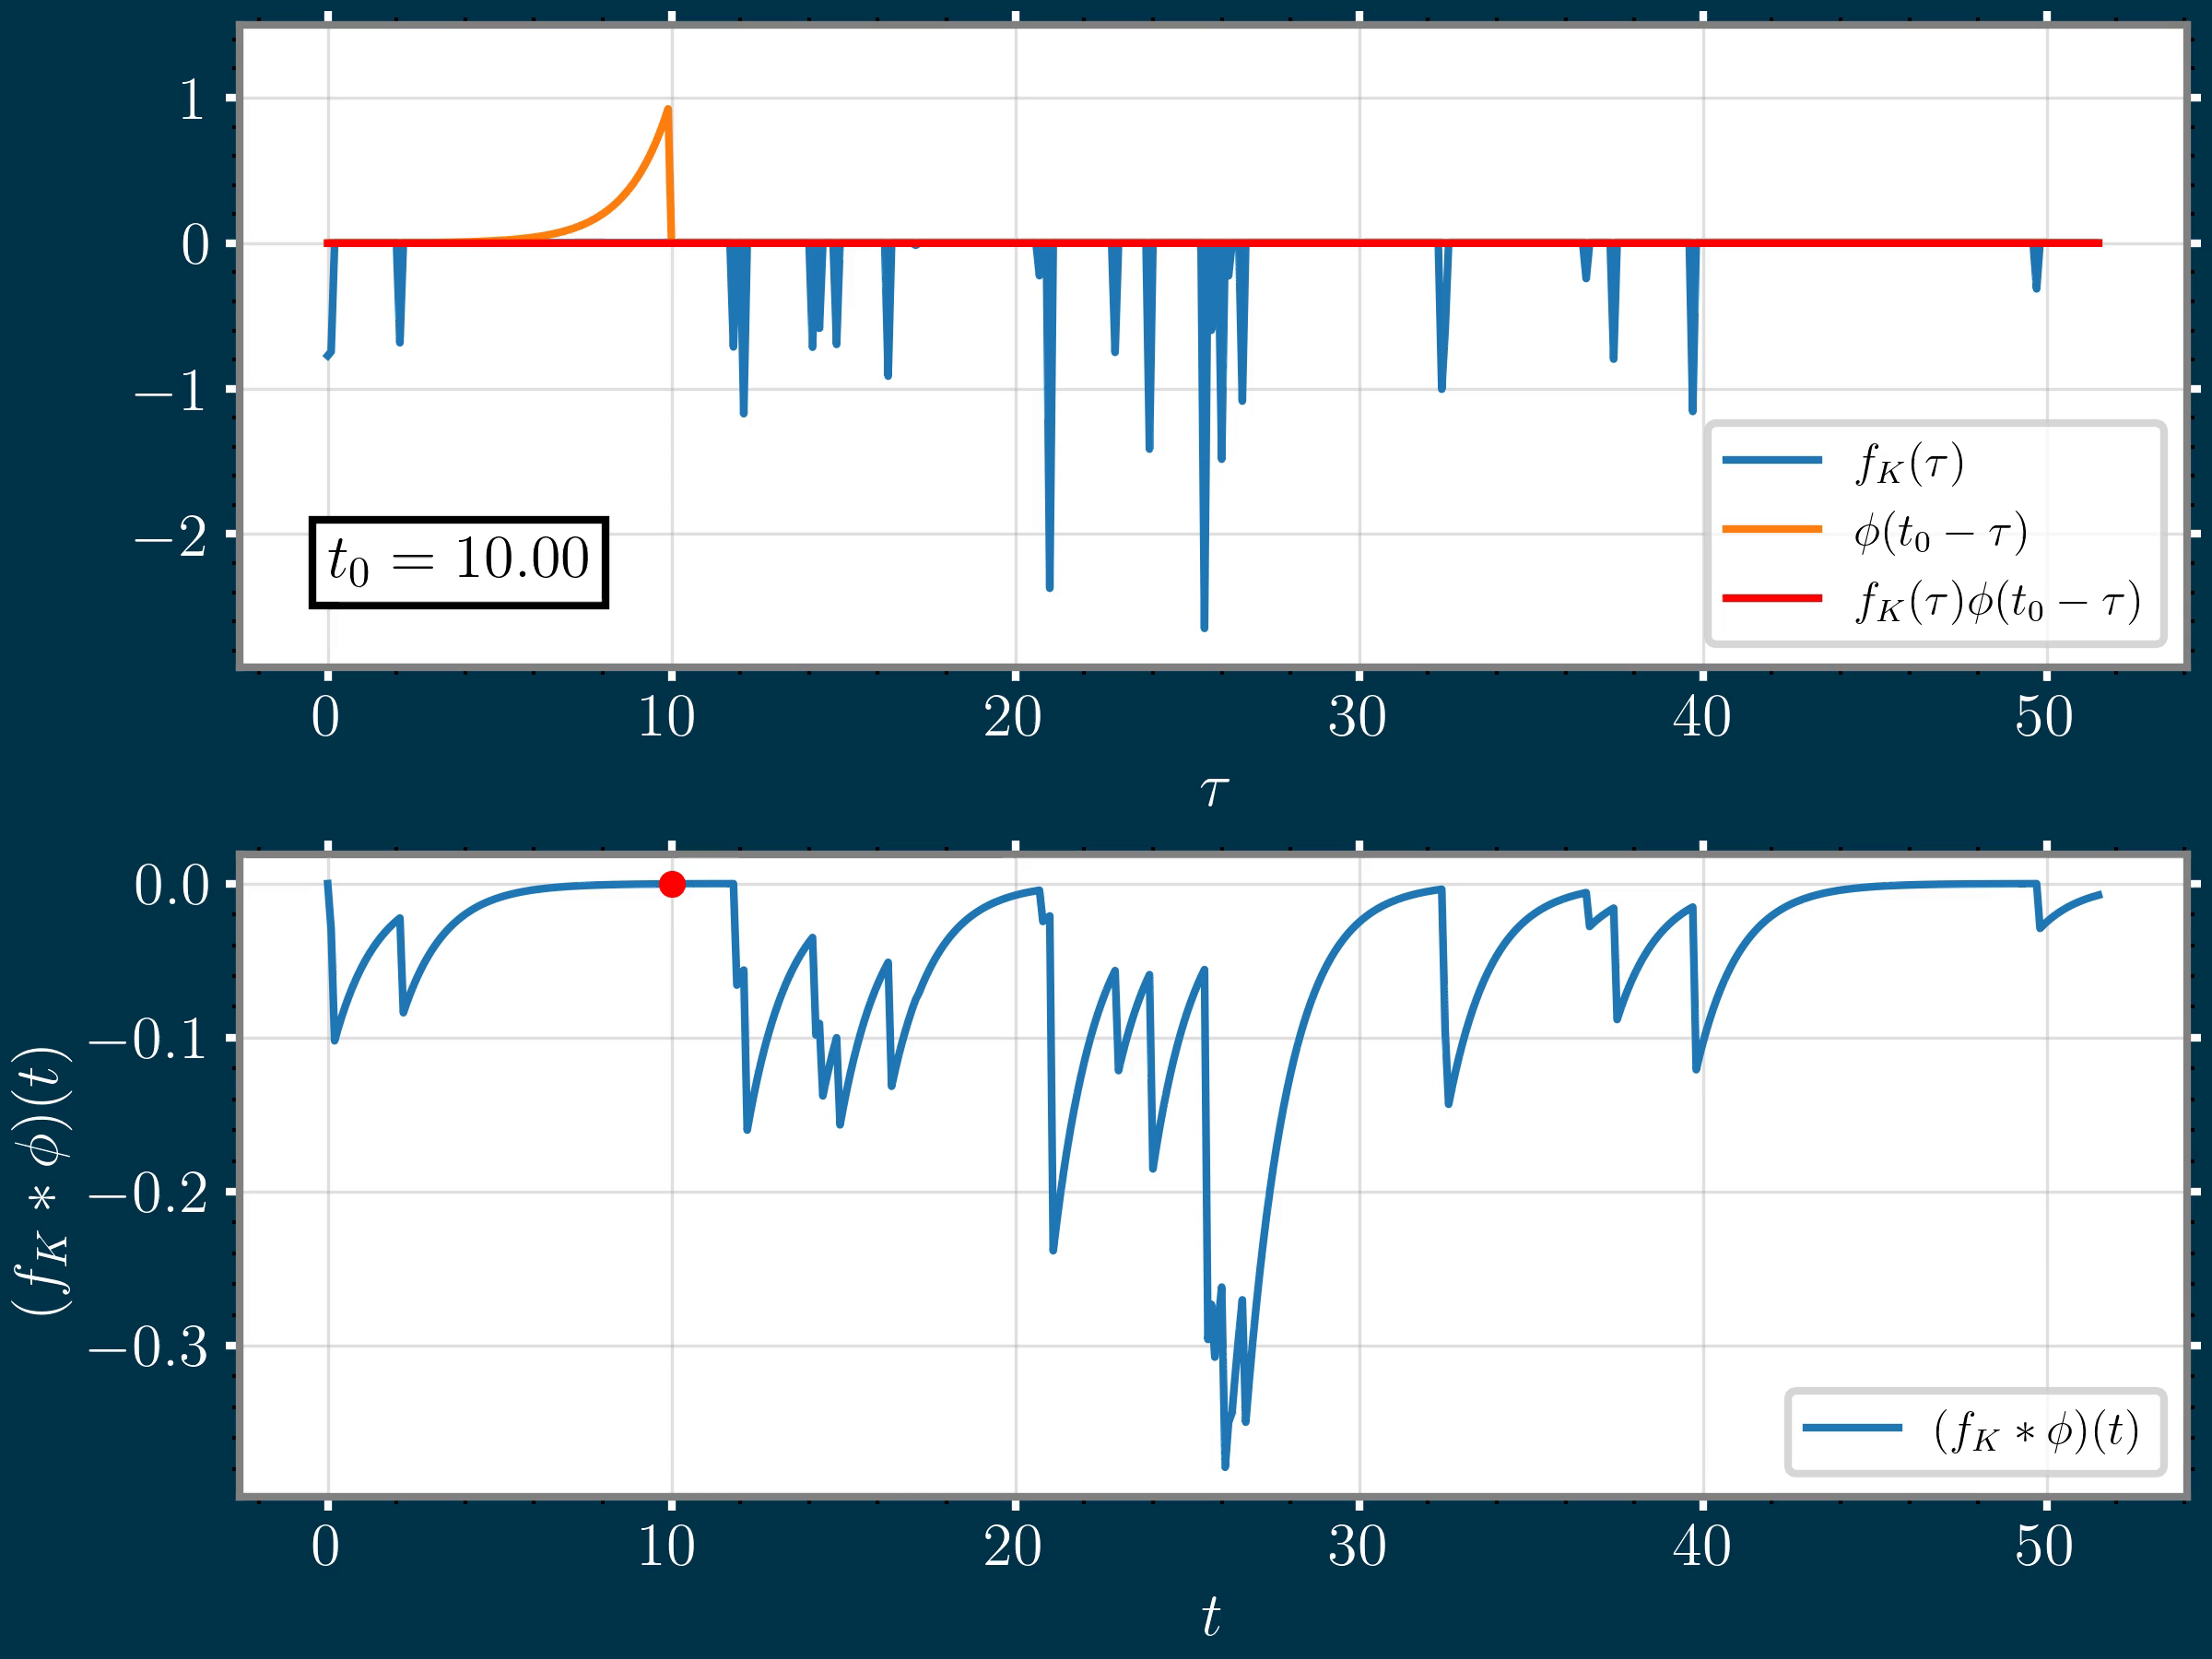
\includegraphics[width=.8\linewidth]{anim.png}
            \end{figure}
        \end{column}
    \end{columns}

    \note<+>{
        \begin{itemize}
            \item So let us look more closely at the FPP
            \item Superpos of individual volcanic events\ldots
        \end{itemize}
    }
    \note<+>{\ldots where each pulse has some amplitude \(A_k\)\ldots}
    \note<+>{\ldots they arrive according to a Poisson process at times \(t_k\)\ldots}
    \note<+>{\ldots and their duration is constant, given as \(\tau_\mathrm{d}\)}
    \note<+>{
        \begin{itemize}
            \item Can be written up as a convolution equation, where a common pulse
                shape is convolved with a forcing, which is also a sum of individual
                pulses, interpreted as volcanic eruptions
            \item We se in the animation how the convolution is done
            \item This assumes knowledge about the response function and the
                forcing, which gives you temperature as the output, so we need a method
                of turning it around
        \end{itemize}
    }

\end{frame}

% \begin{frame}{Simple raycasting animation}
%     \animategraphics[controls,loop,autoplay]{1}{conv-}{0}{16}
% \end{frame}

\begin{frame}{Filtered Poisson process --- Definition}

    The underlying phenemenological model:

    \begin{columns}
        \begin{column}{.51\linewidth}
            % \begin{equation}\label{eq:fpp_sum}
            %   % \alt<2>{T_K(t)}{\Phi_K(t)}=\sum_{k=1}^{\alt<2>{K}{K(T)}} A_k \phi\left(\frac{t-t_k}{\tau_\mathrm{d}}\right)
            %   T_K(t)=\sum_{k=1}^{K} A_k \phi\left(\frac{t-t_k}{\tau_\mathrm{d}}\right)
            % \end{equation}
            % \begin{equation*}
            %   \downarrow
            % \end{equation*}
            \begin{equation}\tag{\ref{eq:fpp_convolve}}
                % \alt<2>{T_K(t)}{\Phi_K(t)}=[\phi * f_K]\left(\frac{t}{\tau_\mathrm{d}}\right)
                T_K(t)=[\phi * f_K]\left(\frac{t}{\tau_\mathrm{d}}\right)
            \end{equation}
        \end{column}
        \begin{column}{.65\linewidth}
            \begin{center}
                % \animategraphics[autoplay,loop,width=.8\linewidth]{10}{gif/conv-}{0}{16}
                % 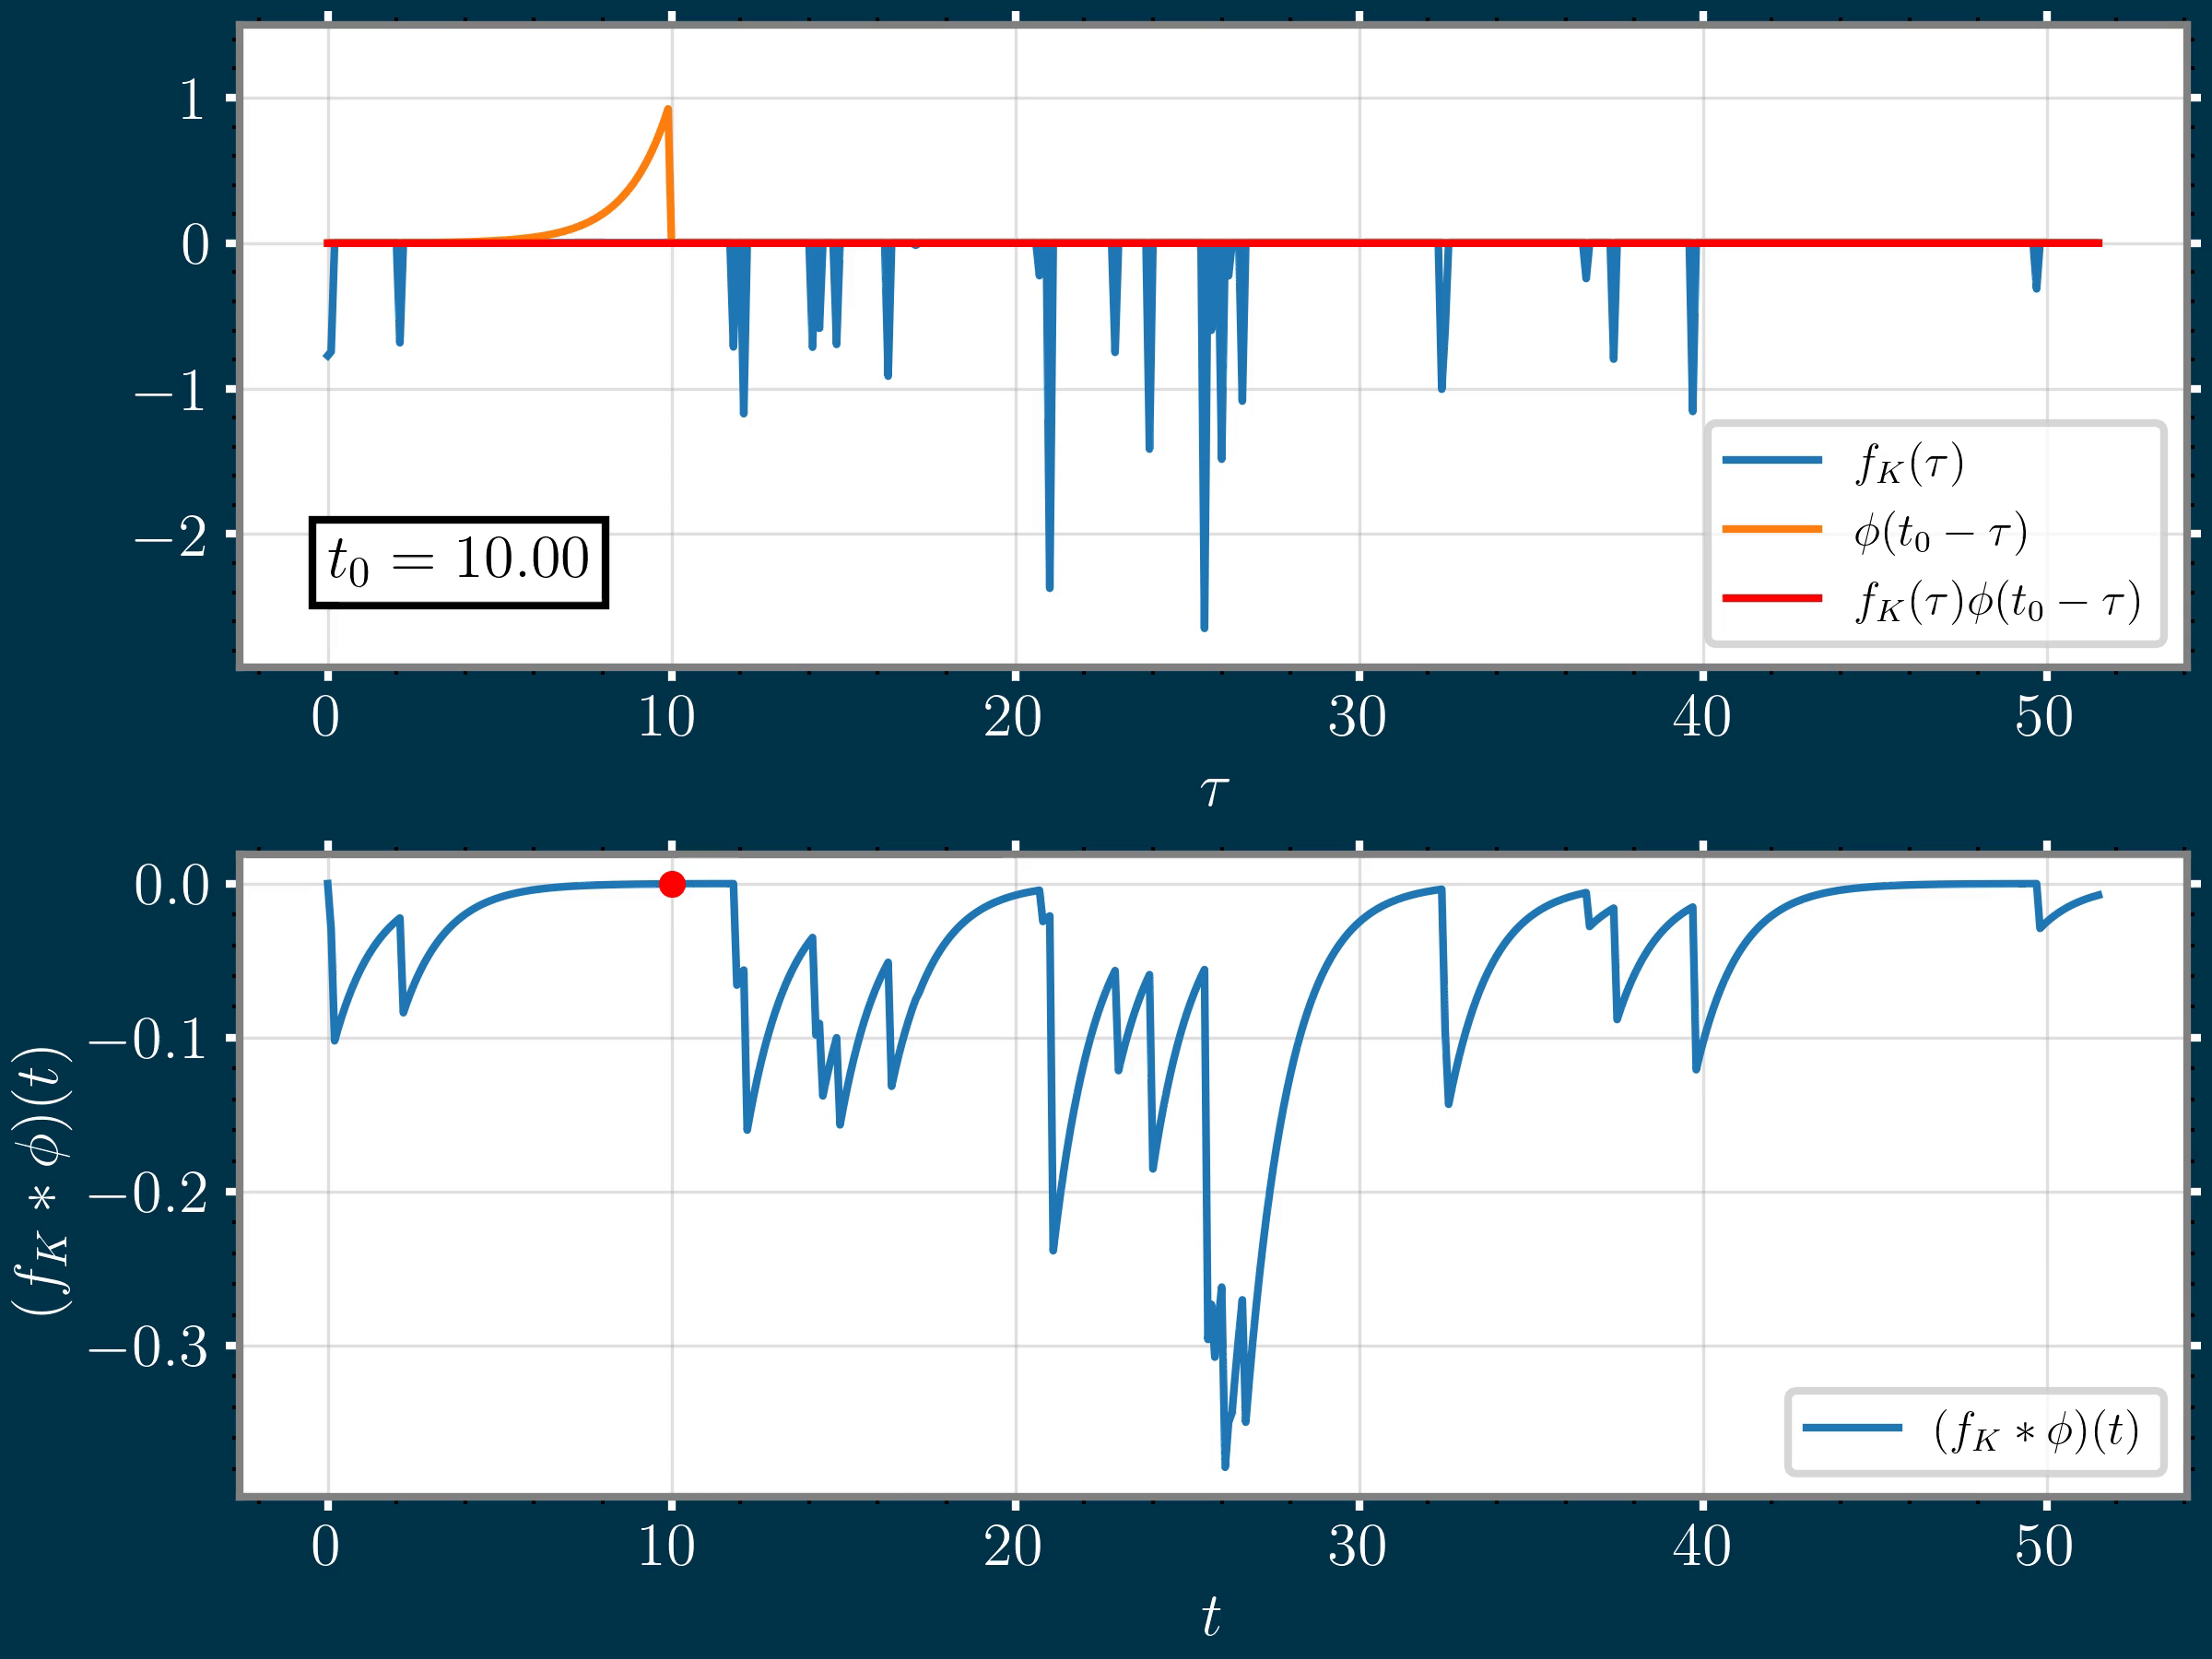
\includegraphics[width=.8\linewidth]{anim.png}
                \movie[
                height=.6\linewidth,
                width=.8\linewidth,
                autostart,
                loop
                ]{}{animation.mp4}
            \end{center}
        \end{column}
    \end{columns}

    \note<+>{
        \begin{itemize}
            \item So let us look more closely at the FPP
            \item Superpos of pulses with amplitudes \(A_k\), arrive according to a
                Poisson process at times \(t_k\) and their duration is constant:
                \(\tau_\mathrm{d}\)
            \item Can be written up as a convolution equation, where a common pulse
                shape is convolved with a forcing, which is also a sum of individual
                pulses, interpreted as volcanic eruptions
            \item We see in the animation how the convolution is done
            \item This assumes knowledge about the response function and the
                forcing, which gives you temperature as the output, so we need a method
                of turning it around
        \end{itemize}
    }

\end{frame}
% \begin{frame}
%   \frametitle{Filtered Poisson process --- Definition}

%   The underlying phenemenological model:

%   \begin{columns}
%     \begin{column}{.51\linewidth}
%       \begin{overprint}
%       \onslide<1>
%         \begin{equation}\label{eq:fpp_sum}
%           % \alt<2>{T_K(t)}{\Phi_K(t)}=\sum_{k=1}^{\alt<2>{K}{K(T)}} A_k \phi\left(\frac{t-t_k}{\tau_\mathrm{d}}\right)
%           \Phi_K(t)=\sum_{k=1}^{K(T)} A_k \phi\left(\frac{t-t_k}{\tau_\mathrm{d}}\right)
%         \end{equation}
%         \begin{equation*}
%           \downarrow
%         \end{equation*}
%         \begin{equation}\label{eq:fpp_convolve}
%           % \alt<2>{T_K(t)}{\Phi_K(t)}=[\phi * f_K]\left(\frac{t}{\tau_\mathrm{d}}\right)
%           \Phi_K(t)=[\phi * f_K]\left(\frac{t}{\tau_\mathrm{d}}\right)
%         \end{equation}
%       \onslide<2>
%       \begin{equation}\tag{\ref{eq:fpp_sum}}
%           % \alt<2>{T_K(t)}{\Phi_K(t)}=\sum_{k=1}^{\alt<2>{K}{K(T)}} A_k \phi\left(\frac{t-t_k}{\tau_\mathrm{d}}\right)
%           T_K(t)=\sum_{k=1}^{K} A_k \phi\left(\frac{t-t_k}{\tau_\mathrm{d}}\right)
%         \end{equation}
%         \begin{equation*}
%           \downarrow
%         \end{equation*}
%         \begin{equation}\tag{\ref{eq:fpp_convolve}}
%           % \alt<2>{T_K(t)}{\Phi_K(t)}=[\phi * f_K]\left(\frac{t}{\tau_\mathrm{d}}\right)
%           T_K(t)=[\phi * f_K]\left(\frac{t}{\tau_\mathrm{d}}\right)
%         \end{equation}
%       \end{overprint}
%     \end{column}
%     \begin{column}{.65\linewidth}
%       \begin{center}
%         \movie[
%           height=.6\linewidth,
%           width=.8\linewidth,
%           autostart,
%           loop
%           ]{}{animation.mp4}
%       \end{center}
%       % \begin{figure}
%       %   \centering
%       %   \animategraphics[autoplay,loop,width=\linewidth]{10}{../figures/deconvolution_anim/deconvolution_}{0}{52}
%       % \end{figure}
%     \end{column}
%   \end{columns}

% \end{frame}

% \begin{frame}
%   \frametitle{Filtered Poisson process --- Definition}

%   \begin{equation}\tag{\ref{eq:fpp_convolve}}
%     T_K(t)=[\phi * f_K]\left(\frac{t}{\tau_\mathrm{d}}\right)
%   \end{equation}

%   Given:
%   \begin{itemize}
%     \item \(\tau_\mathrm{d}\) is constant
%     \item \(f_K\) is a train of delta pulses:
%       \begin{equation}
%         f_K(t)=\sum_{k=1}^{K} A_k\delta\left(\frac{t-t_k}{\tau_\mathrm{d}}\right)
%       \end{equation}
%   \end{itemize}

% \end{frame}

\subsection{Deconvolution}

\begin{frame}{Richardson-Lucy deconvolution}

    An iterative process: \cite{Lucy1974,1972richardson,benvenuto2009}
    \begin{equation}\label{eq:deconvolution}
        \phi^{(n+1)}=\phi^{(n)} \frac{(T_K-\langle T_K\rangle)*\hat{f}_K+b}{\phi^{(n)}*f_K*\hat{f}_K+b}
    \end{equation}

    \note<+>{
        \begin{itemize}
            \item We write up a deconvolution equation, which is an iterative
                algorithm that can take forcing and temperature as the input, and out
                comes the response function
            \item The constant \(b\) regularises the process, ensuring positive
                definite response function
            \item Sajidah spent time discussing this algorithm and considerations
                that are important to account for
            \item It is not trivial, but we will simply apply it in this presentation
        \end{itemize}
    }

\end{frame}

\subsection{Data set}

\begin{frame}{NorESM}

    \(1000\) year long simulation run from the \alert{Norwegian Earth System Model
    (NorESM)}

    \begin{figure}
        \centering
        \includegraphics[width=\linewidth]{noresm/noresm_raw_dark.pdf}
        % \only<1>{\inputpgf[.5]{../figures/noresm.pgf}}
        % \only<2>{\inputpgf[.5]{../figures/noresm_zoom.pgf}}
    \end{figure}

    \note<+>{
        \begin{itemize}
            \item The dataset that is used is from the NorESM, with 1000 year long
                simulation of temperature respons to volcanic forcing
            \item Note the difference in the left and right axis, a factor ten difference
            \item The temperature is monthly resolved while the forcing is yearly resolved
        \end{itemize}
    }

\end{frame}

% How forcing is sampled from yearly to monthly
% \newcounter{prep_note_count}
% \begin{frame}{Preparing NorESM data}

%     \begin{figure}
%         \centering
%         % \inputpgf{../figures/noresm_frc_dark.pgf}
%         \includegraphics[width=\linewidth]{../figures/noresm_frc_dark.pdf}
%     \end{figure}

%     \note{
%         Two approaches:
%         \begin{enumerate}
%             \item Expand forcing by repeating elements to monthly resolution (original is the dotted signal)
%                 \setcounter{prep_note_count}{\value{enumi}}
%         \end{enumerate}
%     }

% \end{frame}

% \begin{frame}
%   \frametitle{Historical forcing data}

%   Forcing data from \cite{jones2004} %and \cite{crowley2003}
%   over the last two millennia

%   \begin{figure}
%     \centering
%     % \inputpgf{../figures/jonesmann.pgf}
%     \includegraphics[width=\linewidth]{../figures/jonesmann.pdf}
%   \end{figure}

% \end{frame}

% \begin{frame}
%   \frametitle{Historical temperature data}

%   Temperature data from \cite{2019_pages2k} over the last two millennia

%   \begin{figure}
%     \centering
%     % \inputpgf{../figures/pages2k.pgf}
%     \includegraphics[width=\linewidth]{../figures/pages2k.pdf}
%   \end{figure}

% \end{frame}

\begin{frame}{Proxy data}

    Forcing and temperature data from \cite{jones2004} and \cite{2019_pages2k}
    of the last two millennia

    \begin{figure}
        \centering
        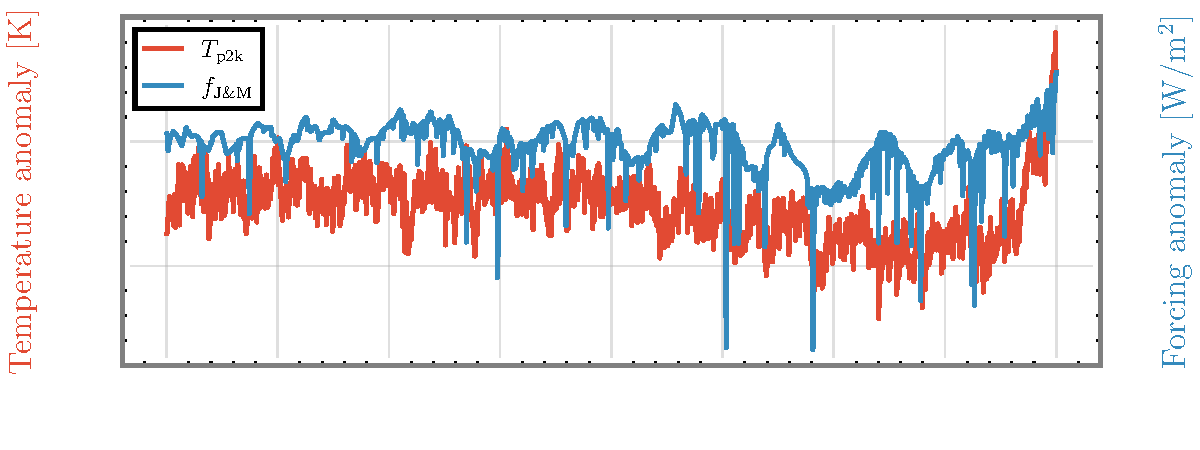
\includegraphics[width=\linewidth]{noresm/raw_historical_beam.pdf}
    \end{figure}

    \note<+>{
        \begin{itemize}
            \item When the response function is obtained, it is tested against
                historical forcing and temperature records inferred from proxy data
            \item Forcing consist of GHG, solar, aerosols, volcanic
            \item Temperature is mean from \(7000\) reconstructions based on proxy data
                from ice cores, tree rings, speleothems, sediments, documentary archives
                and other
        \end{itemize}
    }

\end{frame}


\section{Results}
\subsection{Response function}

\begin{frame}{Response function from deconvolution}

  \begin{figure}
    \centering
    \tikz[baseline]{
      \node[anchor=south] (i1) {\includegraphics[width=.5\linewidth]{noresm/noresm_raw_dark.pdf}};
    }
  \end{figure}

  \vspace{-6mm}
  \begin{center}
    % {\color{MainBlue!35}\textsc{deconvolution}}
    {\pgfsetfillopacity{0.35}
      \textsc{deconvolution}
    }
    \pgfsetfillopacity{1}
  \end{center}\vspace{-6mm}

  \begin{figure}
    \centering
    \tikz[baseline]{
      \node[anchor=south] (o1) {\includegraphics[width=\linewidth]{noresm/response_func_noresm1_choose_dark.pdf}};
    }
  \end{figure}

  \begin{tikzpicture}[overlay]
    \path[->,white] (5.3,6) edge (5.3,5.3);
  \end{tikzpicture}

  \note{
  \begin{itemize}
    \item The solid green line is the result of deconvolution using the NorESM
      dataset, with monthly resolution
    \item The response function is sampled only at whole years, starting
      at \(0, 1, 2, \ldots\)
    \item We re-sample to yearly resolution since the proxy data we want to
      test against have resolution down to one year
  \end{itemize}
  }

\end{frame}

\begin{frame}{Response function from deconvolution}

  \begin{figure}
    \centering
    \tikz[baseline]{
      \node[anchor=south] (i1) {\includegraphics[width=.5\linewidth]{noresm/response_func_noresm1_choose_dark.pdf}};
    }
  \end{figure}

  \vspace{-6mm}
  \begin{center}
    % {\color{MainBlue!35}\textsc{deconvolution}}
    {\pgfsetfillopacity{0.35}
      \textsc{convolution}
    }
    \pgfsetfillopacity{1}
  \end{center}\vspace{-6mm}

  \begin{figure}
    \centering
    \tikz[baseline]{
      \node[anchor=south] (o1) {\includegraphics[width=\linewidth]{noresm/noresm_raw_with_est_dark.pdf}};
    }
  \end{figure}

  \begin{tikzpicture}[overlay]
    \path[->,white] (5.3,6) edge (5.3,5.3);
  \end{tikzpicture}

  \note{
  \begin{itemize}
    \item The solid green line is the result of deconvolution using the NorESM
      dataset, with monthly resolution
    \item The response function is sampled only at whole years, starting
      at \(0, 1, 2, \ldots\)
    \item We re-sample to yearly resolution since the proxy data we want to
      test against have resolution down to one year
  \end{itemize}
  }

\end{frame}

\subsection{Temperature estimates}

\begin{frame}{Temperature of last two millennia}

  \begin{figure}
    \centering%
    \includegraphics[width=\linewidth]{noresm/best_fit_raw_temp1_alone_dark.pdf}%
  \end{figure}

  \note{
  \begin{itemize}
    \item We now look at how well the response function recreates historic
      temperature
    \item The lines are reconstructed temperature and forcing data sets from
      the last two millennia, with temperature in red and forcing in blue (note
      the scale is different by a factor ten)
    \item The response function we obtained is convolved with the blue forcing
      signal, and give an estimated temperature shown as the yellow line
    \item Estimated temperature largely capture the temperature from the forcing
  \end{itemize}
  }

\end{frame}

\begin{frame}{Temperature of \(4\times\ce{CO2}\) experiment}

  \begin{figure}
    \centering
    \includegraphics<1>[width=\linewidth]{estimate_historic/temp_abrupt1_alone_dark.pdf}%
  \end{figure}

  \note{
  \begin{itemize}
    \item Taking a look back at the climate sensitivity, we now convolve the
      response function with a constant forcing representing a quadrupling of
      \ce{CO2} concentration from pre-industrial levels
    \item This is a common experiment to do to decide equilibrium climate
      sensitivity, where the temperature at two different equilibria is
      compared
    \item Able to capture the shape of a NorESM \(4\times\ce{CO2}\) experiment
  \end{itemize}
  }

\end{frame}


\section{Conclusions}
\subsection{Concluding remarks}

\begin{frame}{Concluding remarks}

  \begin{itemize}[<+->]
    \item It is possible to obtain a response function from a
      non-parametric method
    \item Historic temperature is reproduced from forcing data
    \item Reproduces shape of \(4\times\ce{CO2}\) experiment \(\rightarrow\) infer
      climate sensitivity
    % \item Power spectral density of residuals fit nicely to the PSD of a
    %   control run
  \end{itemize}

  \note<1>{
  \begin{itemize}
    \item We saw that it is possible to obtain a response function from a non-parametric method
  \end{itemize}
  }
  \note<2>{
  \begin{itemize}
    \item Using this response function, temperature over the last two millennia
      was reconstructed from forcing data
  \end{itemize}
  }
  \note<3>{
  \begin{itemize}
    \item Finally, using a constant forcing, temperature from a
      \(4\times\ce{CO2}\) experiment was estimated
    \item The estimates had similar shape to the temperature from simulation,
      suggesting the possibility of inferring climate sensitivity from the
      response function
  \end{itemize}
  }

\end{frame}

\subsection{Future work}

\begin{frame}{Future work}

  \begin{itemize}[<+->]
    \item Analysis of the shape of the response function, for example using
      exponentials or power laws
    \item More exact study of the \(4\times\ce{CO2}\) experiment
    \item Effect of clustering of volcanoes
    % \item Estimation of the shape through the deconvolution algorithm using our
    %   own climate simulations
  \end{itemize}
  \vspace{-2mm}
  \begin{figure}
    \centering
    % \includegraphics<1>[width=\linewidth]{../figures/response_func_noresm_all_dark.pdf}
    \includegraphics<1>[width=\linewidth]{../figures/response_func_noresm1_choose_dark.pdf}
    % \includegraphics<2>[width=\linewidth]{../figures/estimate_historic/temp_abrupt1_dark.pdf}%
    \includegraphics<2>[width=\linewidth]{../figures/estimate_historic/temp_abrupt1_alone_dark.pdf}%
    \includegraphics<3->[width=\linewidth]{../figures/raw_historical_beam.pdf}%
    % \includegraphics<3>[width=\linewidth]{../figures/estimate_historic/best_fit_raw_temps_dark.pdf}%
  \end{figure}

  {\pgfsetfillopacity{0.35}
    \begin{tikzpicture}[visible on=<4>,overlay]
    \draw[fill = lightgray] ([xshift=8.46cm,yshift=4.89cm]current page text area.east) rectangle (7.47,1.85);
    \end{tikzpicture}
  }
  \pgfsetfillopacity{1}

  \note<1>{
  \begin{itemize}
    \item Even though the shape is similar in the three versions, it is not
      easy to get an idea of the underlying shape
    \item Settling on one version and investigating what shape it has is one
      future plan
  \end{itemize}
  }
  \note<2>{
  \begin{itemize}
    \item We also saw the constant forcing experiment was well reproduced, but
      this is also short and do not have very high temporal resolution
    \item A more detailed study is therefore sought after
  \end{itemize}
  }
  \note<3>{
  \begin{itemize}
    \item Before the little ice age there are partucularly many strong
      volcanoes, suggesting they might play a role
    \item Studying how such clustering of volcanoes affect climate on longer
      time scales is therefore also included here as future work
  \end{itemize}
  }

\end{frame}


\appendix  % Stops the frame count so the appendix and references are not counted

\begin{frame}[allowframebreaks,plain]{References}

  \begin{footnotesize}
    % \bibliography{/home/een023/science/ref/ref.bib}
    % \bibliographystyle{apalike}  % abbrv
    \printbibliography[heading=none]
  \end{footnotesize}

\end{frame}

% How forcing is sampled from yearly to monthly
\begin{frame}[plain]{Preparing NorESM data}

    \begin{figure}
        \centering
        % \inputpgf{../figures/noresm_frc_dark.pgf}
        \includegraphics[width=\linewidth]{../figures/noresm_frc_dark.pdf}
    \end{figure}

    \note{
        Two approaches:
        \begin{enumerate}
            \item Expand forcing by repeating elements to monthly resolution (original is the dotted signal)
                \setcounter{prep_note_count}{\value{enumi}}
        \end{enumerate}
    }

\end{frame}

\begin{frame}[plain]{Preparing NorESM data}

  \begin{figure}
    \centering
    % \inputpgf{../figures/noresm_temp_dark.pgf}
    \includegraphics[width=\linewidth]{../figures/noresm_temp_dark.pdf}
  \end{figure}

  \note{
    \begin{enumerate}
    \setcounter{enumi}{\value{prep_note_count}}
  \item Or average out temperature to yearly resolution (original is the solid signal)
  \end{enumerate}
  }

\end{frame}

\begin{frame}[plain]{Re-sample response function}

  \begin{figure}
    \centering
    \tikz[baseline]{
      \node[anchor=south] (n1) {\includegraphics[width=.5\linewidth]{../figures/noresm_raw_dark.pdf}};
    }
  \end{figure}

  \vspace{-7mm}
  \begin{center}
    % {\color{MainBlue!35}\textsc{deconvolution}}
    {\pgfsetfillopacity{0.35}
      \textsc{deconvolution}
    }
    \pgfsetfillopacity{1}
  \end{center}\vspace{-3mm}

  \begin{tikzpicture}[remember picture]
    \node[align=top] (t1) {\includegraphics[width=\linewidth]{../figures/response_func_noresm_all_dark.pdf}};
  \end{tikzpicture}

  \begin{tikzpicture}[overlay]
    \path[->,white]<2> (n1) edge (2,5); %(t1.north west);
    \path[->,white]<3> (n1) edge (5.4,5); %(t1.north);
    \path[->,white]<4> (n1) edge (9,5); %(t1.north east);
  \end{tikzpicture}

  \note<+>{
  \begin{itemize}
    \item Due to re-sampling of the forcing and temperature signals, we create
      the response function in three different ways
    \item The solid green lines are the result of deconvolution using the
      NorESM dataset, with A and B coming from monthly resolved data and C from
      yearly resolved data
  \end{itemize}
  }
  \note<+>{
  \begin{itemize}
    \item In A, the response function is sampled only at whole years, starting
      at \(0, 1, 2, \ldots\)
  \end{itemize}
  }
  \note<+>{
  \begin{itemize}
    \item In B, the response function is sampled by doing a forward mean over
      twelve data points, that is, over the months in a year
    \item The value of the yearly resolved response function at year zero is
      the mean of all twelve months from the monthly resolved response function
  \end{itemize}
  }
  \note<+>{
  \begin{itemize}
    \item In C, the response function from the deconvolution already have
      yearly resolution and is only scaled by \(a_0\)
    \item We re-sample to yearly resolution since the proxy data we want to
      test against have resolution down to one year
  \end{itemize}
  }

\end{frame}

\begin{frame}[plain]{Temperature of last two millennia}

  \begin{figure}
    \centering%
    \includegraphics<1>[width=\linewidth]{../figures/estimate_historic/best_fit_raw_temps_dark.pdf}%
    \includegraphics<2>[width=\linewidth]{../figures/estimate_historic/best_fit_raw_temps2_dark.pdf}%
    \includegraphics<3>[width=\linewidth]{../figures/estimate_historic/best_fit_raw_temps3_dark.pdf}%
  \end{figure}

  \note<+>{
  \begin{itemize}
    \item We first look at how well the response function from A recreates
      historic temperature
    \item These are reconstructed temperature and forcing data sets from the
      last two millennia, with temperature in red and forcing in blue (note the
      scale is different by a factor ten)
    \item The response function we obtained is convolved with the blue forcing
      signal, and give an estimated temperature shown as the yellow line
    \item Estimated temperature largely capture the temperature from the forcing
  \end{itemize}
  }
  \note<+>{
  \begin{itemize}
    \item Using response function B yields similar results
    \item Volcanoes give smaller temperature respone using alternative B
      compared to A, othervise similar trend
  \end{itemize}
  }
  \note<+>{
  \begin{itemize}
    \item Again we see a very similar result is obtained from C, showing the
      consistency of the deconvolution algorithm
    \item How the response functions treat fast events differ, but not the trend
  \end{itemize}
  }

\end{frame}

\begin{frame}[plain]{Temperature of \(4\times\ce{CO2}\) experiment}

  \begin{figure}
    \centering
    % 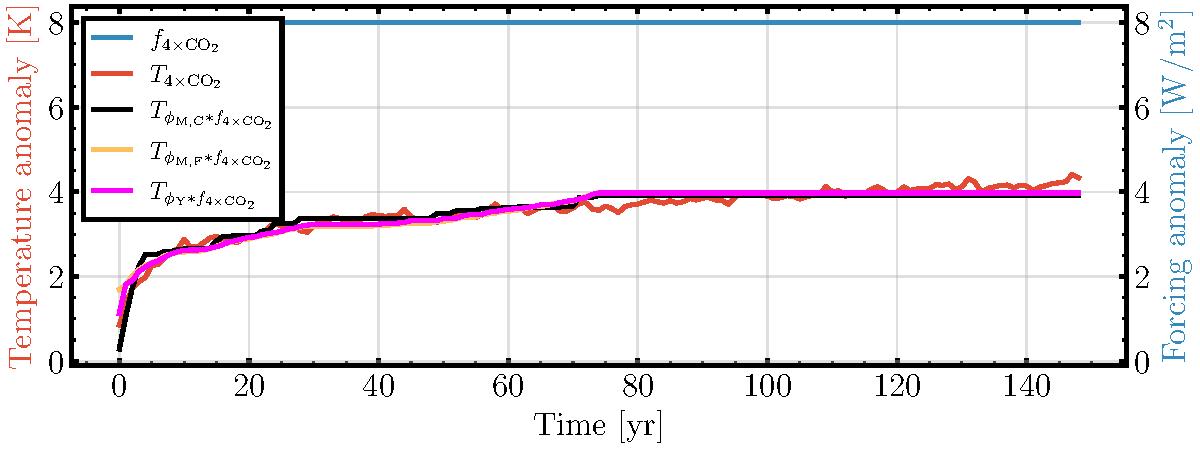
\includegraphics[width=\linewidth]{../figures/estimate_historic/all_temp_abrupt.pdf}%
    \includegraphics<1>[width=\linewidth]{../figures/estimate_historic/temp_abrupt1_dark.pdf}%
    \includegraphics<2>[width=\linewidth]{../figures/estimate_historic/temp_abrupt2_dark.pdf}%
    \includegraphics<3>[width=\linewidth]{../figures/estimate_historic/temp_abrupt3_dark.pdf}%
  \end{figure}

  \note<+>{
  \begin{itemize}
    \item Taking a look back at the climate sensitivity, we now convolve the
      three response functions with a constant forcing representing a
      quadrupling of \ce{CO2} concentration from pre-industrial levels
    \item This is a common experiment to do to decide equilibrium climate
      sensitivity, where the temperature at two different equilibria is
      compared
    \item Able to capture the shape of a NorESM \(4\times\ce{CO2}\) experiment
  \end{itemize}
  }
  \note<+>{
  \begin{itemize}
    \item Compared to a it differ in the first year, but again the response
      function give a temperature estimate that follow the shape of the
      temperature from simulation
  \end{itemize}
  }
  \note<+>{
  \begin{itemize}
    \item Same can be found when using C, first year differ between the three
      versions, but they all capture the trend
  \end{itemize}
  }

\end{frame}

% \subsection{Power spectra}

\begin{frame}[plain]{Power spectra}

  \begin{figure}
    \centering
    \includegraphics[width=\linewidth]{../figures/estimate_historic/all_psd_dark.pdf}
  \end{figure}

  \note<+>{
  \begin{itemize}
    \item The residuals from the estimated historical temperature should have
      same statistics as a simulation without forcing (only noise / internal
      variability)
    \item Good agreement between control run and residuals
  \end{itemize}
  }

\end{frame}


\end{document}
